\chapter{实验}
\section{前言}
在上述内容中,本文分两个章节分别介绍了渐进式多阶段网络框架、基于累积均值平滑的中级监督目标构造方法和基于时空分离策略的Non-Local时空图卷积模块。在上述部分中,本文详细阐述了现有方法的不足与可取之处,进而引出了针对其缺点提出的改进方法,并在给出了本文的解决方案。本章节中,本文希望对本文提出的方法进行定性和定量的分析。具体的,本文将首先介绍渐进式多阶段网络模型的细节。随后将简介实验过程中涉及到的公开数据集,针对各个数据集的特点以及在测试过程中使用的具体设置进行详细的讨论。随后是对实验设置的介绍,包括简述参与对比实验的各个现有方法,实验过程中所使用的对比指标,代码运行的物理环境等等。在完成对实验环境的介绍后,本文将正式进行定量对比实验,即在各个数据集中,不同方法在不同时刻的预测精确性对比。随后对可视化预测结果进行定性的分析。通过预测结果对比证明本方法的高效性后,本文将通过消融实验对网络各部分的设计有效性进行验证。最后是对本方法进行时间效率和空间效率上的分析。

\section{模型实现细节}
\begin{table}[ht]
    % \huge
    \center
    \caption{单阶段网络实现细节}
    \renewcommand\arraystretch{1.2}
    \resizebox{\columnwidth}{!}{
    \begin{tabular}{c|c|c|c|c|c} \hline
    Module                         & \multicolumn{2}{c|}{Layer}                        & Input Size & Operation                 & Output Size \\ \hline
    \multirow{19}{*}{Stage} & \multicolumn{2}{c|}{\multirow{5}{*}{In GCN}}      & (3,22,35) \ding{202} & S-DGCN:A(22,22), W(3,16)  & (16,22,35)  \\ \cline{4-6}
                                  & \multicolumn{2}{c|}{}                             & (16,22,35) & T-DGCN:A(35,35),W(16,16)  & (16,22,35)  \\ \cline{4-6}
                                  & \multicolumn{2}{c|}{}                             & (16,22,35) & BatchNorm                 & (16,22,35)  \\ \cline{4-6}
                                  & \multicolumn{2}{c|}{}                             & (16,22,35) & Tanh                      & (16,22,35)  \\ \cline{4-6}
                                  & \multicolumn{2}{c|}{}                             & (16,22,35) & DropOut:0.3               & (16,22,35)   \\ \cline{2-6}
                                  & \multirow{11}{*}{\makecell*[c]{GCB \\ $\times$ 3}} & \multirow{5}{*}{GCL} & (16,22,35) \ding{203}& S-DGCN:A(22.22), W(16,16) & (16,22,35)  \\ \cline{4-6}
                                  &                           &                      & (16,22,35) & T-DGCN:A(35,35), W(16,16) & (16,22,35)  \\ \cline{4-6}
                                  &                           &                      & (16,22,35) & BatchNorm                 & (16,22,35)  \\ \cline{4-6}
                                  &                           &                      & (16,22,35) & Tanh                      & (16,22,35)  \\ \cline{4-6}
                                  &                           &                      & (16,22,35) & DropOut                   & (16,22,35)  \\ \cline{3-6}
                                  &                           & \multirow{5}{*}{GCL} & (16,22,35) & S-DGCN:A(22.22), W(16,16) & (16,22,35)  \\ \cline{4-6}
                                  &                           &                      & (16,22,35) & T-DGCN:A(35,35), W(16,16) & (16,22,35)  \\ \cline{4-6}
                                  &                           &                      & (16,22,35) & BatchNorm                 & (16,22,35)  \\ \cline{4-6}
                                  &                           &                      & (16,22,35) & Tanh                      & (16,22,35)  \\ \cline{4-6}
                                  &                           &                      & (16,22,35) & DropOut                   & (16,22,35)\ding{204}  \\ \cline{3-6}
                                  &                           & \multicolumn{4}{c}{Residual connection (\ding{203} + \ding{204})}                                     \\ \cline{2-6}
                                  & \multicolumn{2}{c|}{\multirow{2}{*}{Out GCN}}     & (16,22,35) & S-DGCN:A(22.22), W(16,3)  & (3,22,35)   \\ \cline{4-6}
                                  & \multicolumn{2}{c|}{}                             & (3,22,35)  & T-DGCN:A(35,35), W(3,3)   & (3,22,35) \ding{205}  \\ \cline{2-6}
                                  & \multicolumn{5}{c}{Residual connection (\ding{202} + \ding{205})} \\ \hline                                                  
    \end{tabular}
    }
    \label{label:network_structure}
    \end{table}
由于本模型为多阶段模型,为了简便,本文在表\ref{label:network_structure}中只展示了一个阶段的网络模型。若要得到完整的模型只需要对表\ref{label:network_structure}中的结构进行简单的复制即可。除去网络入口的In GCN和出口处的Out GCN部分,整个网络共包含3个GCB(Graph Convolution Block)模块。每个GCB模块又包含两个GCL(Graph Convolution Layer),每个GCL由串联的S-DGCN和T-DGCN,BatchNorm以及DropOut构成。每个GCB内部包含一个横跨输入与输出的残差连接,整个网络又被一个横跨网络输入输出的大的残差连接覆盖,具体的残差连接设计方式请参考表\ref{label:network_structure}。

注意,表\ref{label:network_structure}中的输入和输出数据维度,以及每一层的超参数都是基于模型在Human3.6M数据集上的设置得到的。例如,第三列第二行中输入特征向量的维度为(35,22,3)表示,输入特征是一个长度为35帧的序列(其中前10帧为历史已知序列,由网络输入提供。后25帧为待预测的未来序列,由上一阶段的预测得到(如果当前处于第一个预测阶段,则这部分数据通过复制历史已知序列最后一帧25次得到。))。其中的22表示每个人体姿态由22个关节点构成,每个关节点又由维度为3的特征向量描述。为了满足残差连接中的维度一致性的要求,一个1$\times$1 Convolution layer被用来对输入特征进行特征映射,将原始特征映射到$\mathbb{R}^{35 \times 22 \times 16}$空间中。

此外$W(x,y)$,$A^S(x,y)$,$A^T(x,y)$,$W^S(x,y)$和$W^T(x,y)$中的$x$和$y$代表网络中对应层的权重矩阵维度。例如,在第四列第二行中,S-DGCN空间上邻接矩阵的维度为$\mathbb{R}^{22 \times 22}$,权重矩阵的维度为$\mathbb{R}^{3 \times 16}$。注意网络中的DropOut的遗忘参数被统一设置为0.3。


\section{数据集}
本文分别在Human3.6M\parencite{ionescu2013human3},CMU-MoCap,3DPW\parencite{von2018recovering}这三个数据集上进行测试。

Human3.6M是一个大规模的人体运动捕捉数据集,通常用于与人体运动分析相关的计算机视觉和机器学习研究。它包含超过360万张各种人体运动姿态图像,例如行走、慢跑和蹲下。该数据集是由Max Planck智能系统研究所和英属哥伦比亚大学的研究人员创建的。它使用运动捕捉系统捕捉了附着在人体上的标记的运动。该数据集包括15个不同的人体主体,每个人都执行了17种不同的活动。Human3.6M数据集特别适用于人体姿势估计、动作识别和3D重建等领域的研究。它已被广泛用于各种研究论文,并推动了这些领域的最新技术发展。

本文参考现有工作,挑选出了由7个不同的采样对象贡献的包含15个不同种类的运动数据,其中的7个采集对象的代号为:S1,S5,S6,S7,S8,S9和S11。每个人体姿态由32个以$Exponcntial \ map$格式存储的关节点构成。由于本文主要研究3D空间中的人体运动,因此本文将$Exponcntial map$格式转化为3D格式。此外由于原始数据中存在冗余关节点,即不同编号的关节点位置重合。因此本文去除了10个冗余的关节点。同时,与现有方法一样,本文去除了运动姿态的整体旋转和移动,将视频帧率从50FPS均匀下采样到25FPS。在数据集划分上,采样对象S5贡献的数据作为测试集,S11被用于验证集,其余的数据全部作为训练集。
%酌情添加256,8的实验结果。

CMU-Mocap数据集,也称为卡内基梅隆大学运动捕捉数据集,是由卡内基梅隆大学的运动捕捉实验室创建的一组大型和全面的运动捕捉数据。该数据集包含超过2600个运动捕捉序列,这些序列使用光学运动捕捉系统记录,包括各种人类运动。CMU-Mocap数据集包括各种活动的运动捕捉数据,例如步行、奔跑、跳跃和跳舞。该数据集还包括不同主体的运动捕捉数据,包括男性和女性成年人以及儿童。CMU-Mocap数据集中的运动捕捉数据以多种格式提供,包括C3D、BVH和ASF/AMC。此外,该数据集还包括有关运动捕捉设置和校准的详细信息,以及有关主体和执行的活动的信息。CMU-Mocap数据集已被广泛用于计算机图形学、动画、机器人和生物力学等领域的研究和开发。

CMU-Mocap数据集包含8个人体运动类型,每个人体姿态包含38个关节点,每个关节点的数据格式与Human3.6M类似,为$Exponcntial / map$。同样的本文将其转化为3D格式。运动序列中的整体旋转和移动也被同时去除。在冗余关节点清除上,参考\parencite{dang2021msr,mao2019learning},最终每个人体姿态只保留了25个关节点,其余关节点则被去除。数据集分割策略同样参考\parencite{dang2021msr,mao2019learning},数据集被分割为训练集,测试集和验证集。

3D People in the Wild(3DPW)数据集是一个大规模的自然环境下的3D姿态估计和跟踪基准数据集。该数据集由60个序列组成,包含超过51,000个帧,使用高质量的多摄像头设置在室内外环境中进行捕捉。数据集包括多种活动,例如走路、跳舞和运动,由不同身材、着装和光照条件的多个被试者进行演练。3DPW数据集提供了2D和3D真值标注,包括2D关节位置、相机参数和世界坐标系下的3D人体姿态。使用多视图立体重建来重建3D姿态,通过将参数化人体模型拟合到3D重建中获得地面实况标注。该数据集被广泛应用于评估和开发3D人体姿态估计、3D跟踪和其他相关计算机视觉任务。

对于人体运动姿态预测问题,3DPW是一个十分具有挑战性的数据集。因为它同时包含相对稳定、环境因素简单的室内场景和情况较为复杂的室外场景。与前两个数据集不同,该数据集中的人体运动姿态序列以3D的形式存储,每个人体姿态由26个关节点构成,参考现有方法,本文去掉了前3个冗余的关节点,最终只保留了23个关节点。

\section{实验设置}
\subsection{参与实验的现有方法}
%Res.Sup,DMGNN,LTD,STS-GCN,MSR,Our
在接下来的实验部分中,本文将与Res. Sup.\parencite{martinez2017human},DMGNN\parencite{li2020dynamic},LTD\parencite{mao2019learning},STS-GCN\parencite{sofianos2021space} 和 MSR\parencite{dang2021msr}。Res. Sup.是一个纯RNN结构的方法,DMGNN使用GCN对人体姿态空间结构进行建模,使用RNN进行时间序列建模。LTD则完全依赖GCN,且在频率域对数据进行建模。STS-GCN提出了一种时空分离的时空GCN,但在细节思路上与本文有所不同。MSR则使用了一种空间维度上的渐进式预测策略。以上所有方法均提供公开代码且预测结果达到SOTA。为了公平对比,本文使用它们的预训练模型或在它们的公开代码上使用默认的超参数进行训练。
\subsection{定量对比指标}
本文使用MPJPE(Mean Per-Joint Position Error)作为评价模型预测精确程度的指标。MPJPE代表平均关节点位置误差,用于评估3D人体姿态预测模型性能。它测量预测的3D关节点位置与真实的3D关节点位置之间的平均距离,覆盖数据集中的所有关节点和所有帧。MPJPE是最为通用的度量标准,因为它易于计算和解释,并提供简单的定量测量3D姿态估计的准确性方案。较低的MPJPE值表示姿态估计模型的性能更好,而较高的值表示性能更差。MPJPE被定义为公式\ref{equation:MPJPE}。

\begin{equation}
    MPJPE = \frac{1}{VT}\sum_{i=1}^{V}\sum_{j=1}^{T} | \mathbf{p}_{ij} - \mathbf{p}^{GT}_{ij} |^2
    \label{equation:MPJPE}
\end{equation}

其中$V$是关节点的数量,$T$是帧数,$\mathbf{p}_{ij}$是第$i$个关节点在第$j$帧中的预测3D位置,$\mathbf{p}^{GT}_{ij}$是第$i$个关节点在第$j$帧中的真实3D位置,$|\cdot|^2$表示欧几里得距离。$VT$表示数据集中的关节点和帧数总数。MPJPE通过统计每个关节点预测值和真实值之间的平均误差来度量预测精确性。注意本文只在未知待预测运动序列上计算MPJPE,而非对整个输出序列。例如,假如输入网络的数据长度为35帧,前10帧为已知历史运动序列,后25帧为待预测的未来序列,本文只在后25帧上计算MPJPE。

\subsection{超参数设置和实验环境}
本文的多阶段网络包含4个阶段,每个阶段共包含3个GCB以及入口和出口处的ST-DGCN网络。网络中共计包含12个GCB模块。本文使用$Adam$作为求解器,学习率被初始化为0.005,随后在训练过程中以每个epoch 0.96的递减率下降。训练过程总共包含50个epoch,训练时batchsize为16。本文在NVIDIA RTX 2060 GPU和AMD Ryzen 5 3600 CPU的设备上进行测试。

在网络输入输出格式上,本文参考现有方法,在Human3.6M和CMU-Mocap数据集上输入10帧预测25帧,在3DPW上,输入10帧预测未来30帧。

需要注意的是,对于Human3.6M数据集,本文发现现有方法采用了独特的测试方式。由于Human3.6M数据集中各运动样本数量有细微差距,部分方法选择在每个运动中采样固定数据量的样本作为测试数据集。具体的,\parencite{li2020dynamic, mao2019learning, martinez2017human}从每个动作中采样8个样本,而\parencite{mao2020history}从每个动作中采样256个样本。本文认为上述采样方式虽然可以确保每个动作提供的样本数量一致,但大大减小的测试数据集的规模,导致模型在该数据集上的表现不稳定。同时,Human3.6M中各运动样本数量差距并不悬殊,因此本文沿用了MSR\parencite{dang2021msr}的做法,不进行采样操作,使用全部的测试数据集。为了公平对比,本文也提供了采样数据集上的预测对比,结果显示,本文的优势并没有被削弱。



\section{预测误差对比}\label{section:prediction_error}
\subsection{Human3.6}

\begin{table*}[t]

    \caption{Human3.6M上的短时预测误差对比}
    \renewcommand\arraystretch{0.8}
    \resizebox{\textwidth}{!}{
    \small
    \begin{tabular}{c|cccc|cccc|cccc}\hline
    scenarios   & \multicolumn{4}{c|}{walking}                                   & \multicolumn{4}{c|}{eating}                                    & \multicolumn{4}{c}{smoking}                                   \\ \hline
    millisecond & 80ms          & 160ms         & 320ms         & 400ms         & 80ms          & 160ms         & 320ms         & 400ms         & 80ms          & 160ms         & 320ms         & 400ms         \\ \hline
    Res. Sup.   & 29.4          & 50.8          & 76.0          & 81.5          & 16.8          & 30.6          & 56.9          & 68.7          & 23.0          & 42.6          & 70.1          & 82.7          \\
    DMGNN       & 17.3          & 30.7          & 54.6          & 65.2          & 11.0          & 21.4          & 36.2          & 43.9          & 9.0           & 17.6          & 32.1          & 40.3          \\
    
    LTD         & 12.3          & 23.0          & 39.8          & 46.1          & 8.4           & \underline{16.9}    & 33.2          & 40.7          & \underline{7.9}     & \underline{16.2}    & 31.9          & 38.9          \\
    STS-GCN      & 17.3          & 31.7          & 44.7          & 51.5          & 12.7          & 23.9          & 38.4          & 46.1          & 12.7          & 23.7          & 35.6          & 42.7          \\
    MSR         & \underline{12.2}    & \underline{22.7}    & \underline{38.6}    & \underline{45.2}    & \underline{8.4}     & 17.1          & \underline{33.0}    & \underline{40.4}    & 8.0           & 16.3          & \underline{31.3}    & \underline{38.2}    \\
    Our         & \textbf{10.2} & \textbf{19.8} & \textbf{34.5} & \textbf{40.3} & \textbf{7.0}  & \textbf{15.1} & \textbf{30.6} & \textbf{38.1} & \textbf{6.6}  & \textbf{14.1} & \textbf{28.2} & \textbf{34.7} \\ \hline
    scenarios   & \multicolumn{4}{c|}{discussion}                                & \multicolumn{4}{c|}{directions}                                & \multicolumn{4}{c}{greeting}                                  \\ \hline
    millisecond & 80ms          & 160ms         & 320ms         & 400ms         & 80ms          & 160ms         & 320ms         & 400ms         & 80ms          & 160ms         & 320ms         & 400ms         \\ \hline
    Res. Sup.   & 32.9          & 61.2          & 90.9          & 96.2          & 35.4          & 57.3          & 76.3          & 87.7          & 34.5          & 63.4          & 124.6         & 142.5         \\
    DMGNN       & 17.3          & 34.8          & 61.0          & 69.8          & 13.1          & 24.6          & 64.7          & 81.9          & 23.3          & 50.3          & 107.3         & 132.1         \\
    
    LTD         & 12.5          & 27.4          & 58.5          & 71.7          & 9.0           & 19.9          & 43.4          & \underline{53.7}    & 18.7          & 38.7          & 77.7          & 93.4          \\
    STS-GCN      & 17.0          & 34.5          & 61.9          & 74.7          & 13.7          & 28.0          & 48.6          & 58.9          & 23.0          & 45.2          & 81.5          & 96.9          \\
    MSR         & \underline{12.0}    & \underline{26.8}    & \underline{57.1}    & \underline{69.7}    & \underline{8.6}     & \underline{19.7}    & \underline{43.3}    & 53.8          & \underline{16.5}    & \underline{37.0}    & \underline{77.3}    & \underline{93.4}    \\
    Our         & \textbf{10.0} & \textbf{23.8} & \textbf{53.6} & \textbf{66.7} & \textbf{7.2}  & \textbf{17.6} & \textbf{40.9} & \textbf{51.5} & \textbf{15.2} & \textbf{34.1} & \textbf{71.6} & \textbf{87.1} \\ \hline
    scenarios   & \multicolumn{4}{c|}{phoning}                                   & \multicolumn{4}{c|}{posing}                                    & \multicolumn{4}{c}{purchases}                                 \\\hline
    millisecond & 80ms          & 160ms         & 320ms         & 400ms         & 80ms          & 160ms         & 320ms         & 400ms         & 80ms          & 160ms         & 320ms         & 400ms         \\ \hline
    Res. Sup.   & 38.0          & 69.3          & 115.0         & 126.7         & 36.1          & 69.1          & 130.5         & 157.1         & 36.3          & 60.3          & 86.5          & 95.9          \\
    DMGNN       & 12.5          & 25.8          & 48.1          & 58.3          & 15.3          & 29.3          & 71.5          & 96.7          & 21.4          & 38.7          & 75.7          & 92.7          \\
    
    LTD         & 10.2          & 21.0          & 42.5          & 52.3          & 13.7          & 29.9          & \underline{66.6}    & \underline{84.1}    & 15.6          & 32.8          & \underline{65.7}    & \underline{79.3}    \\
    STS-GCN      & 14.5          & 27.8          & 46.6          & 56.6          & 20.2          & 40.9          & 75.5          & 93.3          & 20.6          & 40.4          & 71.3          & 84.8          \\
    MSR         & \underline{10.1}    & \underline{20.7}    & \underline{41.5}    & \underline{51.3}    & \underline{12.8}    & \underline{29.4}    & 67.0          & 85.0          & \underline{14.8}    & \underline{32.4}    & 66.1          & 79.6          \\
    Our         & \textbf{8.3}  & \textbf{18.3} & \textbf{38.7} & \textbf{48.4} & \textbf{10.7} & \textbf{25.7} & \textbf{60.0} & \textbf{76.6} & \textbf{12.5} & \textbf{28.7} & \textbf{60.1} & \textbf{73.3} \\ \hline
    scenarios   & \multicolumn{4}{c|}{sitting}                                   & \multicolumn{4}{c|}{sittingdown}                               & \multicolumn{4}{c}{takingphoto}                               \\ \hline
    millisecond & 80ms          & 160ms         & 320ms         & 400ms         & 80ms          & 160ms         & 320ms         & 400ms         & 80ms          & 160ms         & 320ms         & 400ms         \\ \hline
    Res. Sup.   & 42.6          & 81.4          & 134.7         & 151.8         & 47.3          & 86.0          & 145.8         & 168.9         & 26.1          & 47.6          & 81.4          & 94.7          \\
    DMGNN       & 11.9          & 25.1          & 44.6          & \textbf{50.2} & \underline{15.0}    & 32.9          & 77.1          & 93.0          & 13.6          & 29.0          & 46.0          & 58.8          \\
    
    LTD         & 10.6          & \underline{21.9}    & 46.3          & 57.9          & 16.1          & \underline{31.1}    & \underline{61.5}    & \underline{75.5}    & 9.9           & \underline{20.9}    & 45.0          & 56.6          \\
    STS-GCN      & 16.2          & 30.2          & 52.7          & 65.1          & 23.3          & 41.5          & 69.6          & 83.5          & 16.7          & 31.4          & 52.8          & 64.3          \\
    MSR         & \underline{10.5}    & 22.0          & \underline{46.3}    & 57.8          & 16.1          & 31.6          & 62.5          & 76.8          & \underline{9.9}     & 21.0          & \underline{44.6}    & \underline{56.3}    \\
    Our         & \textbf{8.8}  & \textbf{19.2} & \textbf{42.4} & \underline{53.8}    & \textbf{13.9} & \textbf{27.9} & \textbf{57.4} & \textbf{71.5} & \textbf{8.4}  & \textbf{18.9} & \textbf{42.0} & \textbf{53.3} \\ \hline
    \end{tabular}
    }
    
    \resizebox{\textwidth}{!}{
    \begin{tabular}{c|cccc|cccc|cccc|cccc} \hline
    scenarios   & \multicolumn{4}{c|}{waiting}                                  & \multicolumn{4}{c|}{walkingdog}                                & \multicolumn{4}{c|}{walkingtogether}                          & \multicolumn{4}{c}{average}                                       \\ \hline
    millisecond & 80ms         & 160ms         & 320ms         & 400ms         & 80ms          & 160ms         & 320ms         & 400ms         & 80ms         & 160ms         & 320ms         & 400ms         & 80ms          & 160ms         & 320ms         & 400ms         \\ \hline
    Res. Sup.   & 30.6         & 57.8          & 106.2         & 121.5         & 64.2          & 102.1         & 141.1         & 164.4         & 26.8         & 50.1          & 80.2          & 92.2          & 34.7          & 62.0          & 101.1         & 115.5         \\
    DMGNN       & 12.2         & 24.2          & 59.6          & 77.5          & 47.1          & 93.3          & 160.1         & 171.2         & 14.3         & 26.7          & 50.1          & 63.2          & 17.0          & 33.6          & 65.9          & 79.7          \\
    
    LTD         & 11.4         & 24.0          & 50.1          & 61.5          & 23.4          & 46.2          & 83.5          & 96.0          & \underline{10.5}   & 21.0          & 38.5          & 45.2          & 12.7          & 26.1          & 52.3          & 63.5          \\
    STS-GCN      & 16.1         & 31.9          & 54.0          & 65.2          & 27.8          & 51.5          & 85.0          & 97.4          & 15.3         & 27.8          & 41.2          & 48.0          & 17.8          & 34.0          & 57.3          & 68.6          \\
    MSR         & \underline{10.7}   & \underline{23.1}    & \underline{48.3}    & \underline{59.2}    & \underline{20.7}    & \underline{42.9}    & \underline{80.4}    & \underline{93.3}    & 10.6         & \underline{20.9}    & \underline{37.4}    & \underline{43.9}    & \underline{12.1}    & \underline{25.6}    & \underline{51.6}    & \underline{62.9}    \\
    Our         & \textbf{8.9} & \textbf{20.1} & \textbf{43.6} & \textbf{54.3} & \textbf{18.8} & \textbf{39.3} & \textbf{73.7} & \textbf{86.4} & \textbf{8.7} & \textbf{18.6} & \textbf{34.4} & \textbf{41.0} & \textbf{10.3} & \textbf{22.7} & \textbf{47.4} & \textbf{58.5} \\ \hline
    \end{tabular}
    }
    \label{table:Human3.6M_short-term}
    \end{table*}




    \begin{table*}[ht]
        \caption{ Human3.6M 上的长时预测误差对比。}
        \center
        \renewcommand\arraystretch{1}
        \resizebox{1\textwidth}{!}{
        \small
        \begin{tabular}{c|cc|cc|cc|cc|cc} \hline
        scenarios   & \multicolumn{2}{c|}{walking}     & \multicolumn{2}{c|}{eating}    & \multicolumn{2}{c|}{smoking}     & \multicolumn{2}{c|}{discussion} & \multicolumn{2}{c}{directions} \\ \hline
        millisecond & 560ms          & 1000ms         & 560ms         & 1000ms        & 560ms          & 1000ms         & 560ms         & 1000ms         & 560ms         & 1000ms         \\\hline
        Res. Sup.   & 81.7           & 100.7          & 79.9          & 100.2         & 94.8           & 137.4          & 121.3         & 161.7          & 110.1         & 152.5          \\
        DMGNN       & 73.4           & 95.8           & 58.1          & 86.7          & 50.9           & 72.2           & \textbf{81.9} & 138.3          & 110.1         & 115.8          \\
        LTD         & 54.1           & \underline{59.8}     & 53.4          & 77.8          & 50.7           & 72.6           & 91.6          & 121.5          & \underline{71.0}    & 101.8          \\
        STS-GCN      & 56.3           & 69.1           & 59.3          & 84.3          & 53.3           & 75.4           & 93.0          & 121.8          & 75.5          & 104.8          \\
        MSR         & \underline{52.7}     & 63.0           & \underline{52.5}    & \underline{77.1}    & \underline{49.5}     & \underline{71.6}     & 88.6          & \textbf{117.6} & 71.2          & \underline{100.6}    \\
        Our         & \textbf{48.1}  & \textbf{56.4}  & \textbf{51.1} & \textbf{76.0} & \textbf{46.5}  & \textbf{69.5}  & \underline{87.1}    & \underline{118.2}    & \textbf{69.3} & \textbf{100.4} \\ \hline
        scenarios   & \multicolumn{2}{c|}{greeting}    & \multicolumn{2}{c|}{phoning}   & \multicolumn{2}{c|}{posing}      & \multicolumn{2}{c|}{purchases}  & \multicolumn{2}{c}{sitting}    \\ \hline
        millisecond & 560ms          & 1000ms         & 560ms         & 1000ms        & 560ms          & 1000ms         & 560ms         & 1000ms         & 560ms         & 1000ms         \\ \hline
        Res. Sup.   & 156.1          & 166.5          & 141.2         & 131.5         & 194.7          & 240.2          & 122.7         & 160.3          & 167.4         & 201.5          \\
        DMGNN       & 152.5          & 157.7          & 78.9          & \textbf{98.6} & 163.9          & 310.1          & 118.6         & 153.8          & \textbf{60.1} & \textbf{104.9} \\
        LTD         & \underline{115.4}    & 148.8          & 69.2          & 103.1         & \underline{114.5}    & \underline{173.0}    & 102.0         & 143.5          & 78.3          & 119.7          \\
        STS-GCN      & 117.6          & \underline{145.6}    & 73.3          & 108.5         & 122.4          & 175.1          & 104.8         & 140.8          & 86.0          & 124.3          \\
        MSR         & 116.3          & 147.2          & \underline{68.3}    & 104.4         & 116.3          & 174.3          & \underline{101.6}   & \underline{139.2}    & 78.2          & 120.0          \\
        Our         & \textbf{110.2} & \textbf{143.5} & \textbf{65.9} & \underline{102.7}   & \textbf{106.1} & \textbf{164.8} & \textbf{95.3} & \textbf{133.3} & \underline{74.4}    & \underline{116.1}   \\ \hline
        \end{tabular}
        }
        
        \resizebox{1\textwidth}{!}{
        \begin{tabular}{c|cc|cc|cc|cc|cc|cc} \hline
        scenarios   & \multicolumn{2}{c|}{sittingdown} & \multicolumn{2}{c|}{takingphoto} & \multicolumn{2}{c|}{waiting}    & \multicolumn{2}{c|}{walkingdog}  & \multicolumn{2}{c|}{walkingtogether} & \multicolumn{2}{c}{average}    \\ \hline
        millisecond & 560ms          & 1000ms         & 560ms          & 1000ms         & 560ms         & 1000ms         & 560ms          & 1000ms         & 560ms            & 1000ms           & 560ms         & 1000ms         \\ \hline
        Res. Sup.   & 205.3          & 277.6          & 117.0          & 143.2          & 146.2         & 196.2          & 191.3          & 209.0          & 107.6            & 131.1            & 97.6          & 130.5          \\
        DMGNN       & 122.1          & 168.8          & 91.6           & 120.7          & 106.0         & 136.7          & 194.0          & 182.3          & 83.4             & 115.9            & 103.0         & 137.2          \\
        LTD         & \underline{100.0}    & \underline{150.2}    & \underline{77.4}     & \underline{119.8}    & 79.4          & 108.1          & 111.9          & 148.9          & 55.0             & \underline{65.6}       & 81.6          & 114.3          \\
        STS-GCN      & 107.8          & 157.3          & 85.0           & 125.8          & 81.7          & 112.4          & 114.3          & \underline{146.9}    & 56.1             & 69.8             & 85.7          & 117.5          \\
        MSR         & 102.8          & 155.5          & 77.9           & 121.9          & \underline{76.3}    & \underline{106.3}    & \underline{111.9}    & 148.2          & \underline{52.9}       & 65.9             & \underline{81.1}    & \underline{114.2}    \\
        Our         & \textbf{96.7}  & \textbf{147.8} & \textbf{74.3}  & \textbf{118.6} & \textbf{72.2} & \textbf{103.4} & \textbf{104.7} & \textbf{139.8} & \textbf{51.9}    & \textbf{64.3}    & \textbf{76.9} & \textbf{110.3} \\ \hline
        \end{tabular}
        }
        \label{table:Human3.6long-term}
        \end{table*}

表\ref{table:Human3.6M_short-term}展示了在Human3.6M数据集上的短时预测结果(输入10帧预测10帧,在25FPS的视频中即输入400ms的运动预测400ms的运动。),本文统计了15个运动类别上,80ms,160ms,320ms,400ms四个时刻的平均预测误差,图中预测误差最低的结果被加粗,而第二好的结果被加上了下划线。从表\ref{table:Human3.6M_short-term}可以看到,在全部15个运动类别共60个时刻中,本方法在其中的59个时刻预测误差均为六个方法中的最低,唯一一个落后的时刻也处于第二低的位置。且本方法相较于现有方法在sitting,sittingdown,purchases,walkingdog这些较为复杂的运动上取得了较为明显的领先,这表明了本方法的有效性,在所有运动的平均误差上,本文的结果(10.3,22.7,47.4,58.5)也远远高于第二的MSR(12.1,25.6,51.6,62.9)。

表\ref{table:Human3.6long-term}展示了在Human3.6M数据集上长时预测结果(输入10帧预测25帧,即输入400ms预测1000ms。),与表\ref{table:Human3.6M_short-term}一样,本文统计了15个运动类别上,560ms,1000ms两个时刻的平均预测误差,不同方法间预测误差最低的结果被加粗,第二低的结果添加下划线。在长时预测中,本方法依然在30个时刻中的25个中的得到了最低的预测误差,其余5个非最优结果中,也位于第二优的位置。且由于长时预测中不确定性增加,本方法相较于现有SOTA方法优势更明显,体现了本方法在提取长时依赖能力上的强大。

除了在完整的测试数据集上进行测试,本文还参考\parencite{li2020dynamic, mao2019learning, martinez2017human,mao2020history}分别在每个动作采样8或256个样本的的测试数据集上进行实验。表\ref{table:human3.6_shortterm_256}和表\ref{table:human3.6_longterm_256}分别表示模型在每个动作采样256个样本的测试数据集上的短时和长时预测误差。表\ref{table:human3.6 short-term 8}和表\ref{table:human3.6 long-term 8}分别表示模型在每个动作采样8个样本的测试数据集上的短时和长时预测误差。注意在这两个表中,本文添加与Transformer\parencite{aksan2021spatio}对比的内容,该文章只提供了采样8个样本的预测结果,且在长时预测上存在部分数据缺失的情况,因此本文只使用了论文中提供的结果。从上述对比表格来看,本方法依然延续了在预测精度上的优势。

\clearpage

\begin{table*}[h]
    \caption{Human3.6M上每个动作随机采样256的短时误差对比}
    \renewcommand\arraystretch{0.8}
    \resizebox{\textwidth}{!}{
    \begin{tabular}{c|cccc|cccc|cccc|cccc} \hline
    scenarios   & \multicolumn{4}{c|}{walking}                                   & \multicolumn{4}{c|}{eating}                                    & \multicolumn{4}{c|}{smoking}                                   & \multicolumn{4}{c}{discussion}                               \\\hline
    millisecond & 80ms          & 160ms         & 320ms         & 400ms         & 80ms          & 160ms         & 320ms         & 400ms         & 80ms          & 160ms         & 320ms         & 400ms         & 80ms         & 160ms         & 320ms         & 400ms         \\ \hline
    Res. Sup.   & 23.2          & 40.9          & 61            & 66.7          & 16.8          & 31.5          & 53.5          & 61.7          & 18.9          & 34.7          & 57.5          & 65.4          & 25.7         & 47.8          & 80            & 91.3          \\
    DMGNN & 18.4          & 33.6          & 56.8          & 65.1          & 10.1          & 19.7          & 38.3          & 46.7          & 11.4          & 22.0          & 41.5          & 50.1          & 18.0         & 36.2          & 71.9          & 85.2          \\
    LTD   & 11.1          & 21.4          & 37.3          & 42.9          & 7             & 14.8          & 29.8          & 37.3          & 7.5           & 15.5          & 30.7          & 37.5          & 10.8         & 24            & 52.7          & 65.8          \\
    STS-GCN              & 18.0                 & 32.9                 & 46.7                 & 53.4                          & 12.1                 & 23.3                 & 36.8                 & 44.3                 & 13.0                 & 24.3                 & 37.2                 & 44.6                 & 17.1                 & 33.2                 & 58.6                 & 71.3                 \\
    MSR   & \underline{10.8}          & \underline{20.9}          & \underline{36.9}          & \underline{42.4}          & \underline{6.9}           & \underline{14.6}          & \underline{29.0}          & \underline{36.0}          & \underline{7.5}           & \underline{15.4}          & \underline{30.6}          & \underline{37.5}          & \underline{10.4}         & \underline{23.5}          & \underline{51.9}          & \underline{65.0}          \\ 
    Ours   & \textbf{9.4}  & \textbf{19.0} & \textbf{34.3} & \textbf{40.4} & \textbf{6.0}  & \textbf{13.4} & \textbf{27.8} & \textbf{35.3} & \textbf{6.5}  & \textbf{14.2} & \textbf{28.8} & \textbf{35.5} & \textbf{9.0} & \textbf{21.8} & \textbf{49.9} & \textbf{62.9} \\\hline
    scenarios   & \multicolumn{4}{c|}{directions}                                & \multicolumn{4}{c|}{greeting}                                  & \multicolumn{4}{c|}{phoning}                                   & \multicolumn{4}{c}{posing}                                   \\ \hline
    millisecond & 80ms          & 160ms         & 320ms         & 400ms         & 80ms          & 160ms         & 320ms         & 400ms         & 80ms          & 160ms         & 320ms         & 400ms         & 80ms         & 160ms         & 320ms         & 400ms         \\ \hline
    Res. Sup.   & 21.6          & 41.3          & 72.1          & 84.1          & 31.2          & 58.4          & 96.3          & 108.8         & 21.1          & 38.9          & 66            & 76.4          & 29.3         & 56.1          & 98.3          & 114.3         \\
    DMGNN & 13.8          & 27.7          & 55.3          & 67.2          & 22.6          & 45.1          & 89.0          & 106.6         & 14.3          & 28.0          & 52.4          & 63.3          & 18.6         & 37.6          & 80.1          & 100.0         \\
    LTD   & 8             & \underline{18.8}          & \underline{43.7}          & \underline{54.9}          & \underline{14.8}          & \underline{31.4}          & \underline{65.3}          & \underline{79.7}          & 9.3           & 19.1          & \underline{39.8}          & \underline{49.7}          & 10.9         & 25.1          & \underline{59.1}          & 75.9          \\
    STS-GCN              & 13.9                 & 29.3                 & 52.8                 & 64.0                          & 20.8                 & 40.7                 & 72.2                 & 85.9                 & 14.5                 & 27.3                 & 45.7                 & 55.4                 & 19.0                 & 38.9                 & 71.7                 & 89.2                 \\
    MSR   & \underline{7.7}           & 18.9          & 44.7          & 56.2          & 15.1          & 33.1          & 70.9          & 85.4          & \underline{9.1}           & \underline{18.9}          & 39.9          & 49.8          & \underline{10.3}         & \underline{24.6}          & 59.2          & \underline{75.9}          \\
    Ours   & \textbf{6.4}  & \textbf{16.8} & \textbf{41.5} & \textbf{52.7} & \textbf{12.4} & \textbf{28.3} & \textbf{61.2} & \textbf{76.0} & \textbf{7.8}  & \textbf{17.2} & \textbf{37.3} & \textbf{47.3} & \textbf{8.7} & \textbf{22.2} & \textbf{53.9} & \textbf{70.4} \\ \hline
    scenarios   & \multicolumn{4}{c|}{purchases}                                 & \multicolumn{4}{c|}{sitting}                                   & \multicolumn{4}{c|}{sittingdown}                               & \multicolumn{4}{c}{takingphoto}                              \\ \hline
    millisecond & 80ms          & 160ms         & 320ms         & 400ms         & 80ms          & 160ms         & 320ms         & 400ms         & 80ms          & 160ms         & 320ms         & 400ms         & 80ms         & 160ms         & 320ms         & 400ms         \\ \hline
    Res. Sup.   & 28.7          & 52.4          & 86.9          & 100.7         & 23.8          & 44.7          & 78            & 91.2          & 31.7          & 58.3          & 96.7          & 112           & 21.9         & 41.4          & 74            & 87.6          \\
    DMGNN & 21.7          & 42.4          & 77.3          & 91.6          & 14.7          & 30.0          & 61.5          & 74.5          & 20.7          & 39.9          & 81.0          & 97.4          & 14.4         & 29.2          & 59.4          & 74.6          \\
    LTD   & 13.9          & 30.3          & \underline{62.2}          & \underline{75.9}          & 9.8           & \underline{20.5}          & 44.2          & 55.9          & 15.6          & \underline{31.4}          & \underline{59.1}          & \underline{71.7}          & 8.9          & \underline{18.9}          & \underline{41}            & \underline{51.7}          \\
    STS-GCN              & 20.9                 & 41.4                 & 71.8                 & 86.0                          & 16.0                 & 30.1                 & 51.9                 & 63.9                 & 23.9                 & 42.9                 & 68.9                 & 81.5                 & 16.2                 & 31.3                 & 52.1                 & 63.4                 \\
    MSR   & \underline{13.3}          & \underline{30.1}          & 63.6          & 77.8          & \underline{9.8}           & 20.6          & \underline{44.2}          & \underline{55.5}          & \underline{15.4}          & 32.0          & 60.7          & 73.8          & \underline{8.9}          & 19.5          & 43.1          & 54.4          \\
    Ours   & \textbf{11.7} & \textbf{27.8} & \textbf{59.4} & \textbf{73.5} & \textbf{8.5}  & \textbf{18.8} & \textbf{41.8} & \textbf{53.2} & \textbf{13.7} & \textbf{29.3} & \textbf{57.2} & \textbf{69.7} & \textbf{7.6} & \textbf{17.2} & \textbf{38.5} & \textbf{49.2} \\ \hline
    scenarios   & \multicolumn{4}{c}{waiting}                                   & \multicolumn{4}{c}{walkingdog}                                & \multicolumn{4}{c}{walkingtogether}                           & \multicolumn{4}{c}{average}                                      \\ \hline
    millisecond & 80ms          & 160ms         & 320ms         & 400ms         & 80ms          & 160ms         & 320ms         & 400ms         & 80ms          & 160ms         & 320ms         & 400ms         & 80ms         & 160ms         & 320ms         & 400ms         \\ \hline
    Res. Sup.   & 23.8          & 44.2          & 75.8          & 87.7          & 36.4          & 64.8          & 99.1          & 110.6         & 20.4          & 37.1          & 59.4          & 67.3          & 25           & 46.2          & 77            & 88.3          \\
    DMGNN & 15.5          & 30.7          & 61.5          & 74.4          & 31.7          & 62.1          & 109.8         & 125.3         & 15.7          & 29.2          & 51.1          & 60.7          & 17.4         & 34.2          & 65.8          & 78.9          \\
    LTD   & \underline{9.2}           & \underline{19.5}          & \underline{43.3}          & \underline{54.4}          & \underline{20.9}          & \underline{40.7}          &\underline{73.6}          & \underline{86.6}          & 9.6           & 19.4          & 36.5          & 44            & \underline{11.2}         & \underline{23.4}          & \underline{47.9}          & \underline{58.9}          \\
    STS-GCN              & 15.9                 & 31.5                 & 52.3                 & 63.4                          & 29.2                 & 53.3                 & 84.2                 & 96.1                 & 15.5                 & 28.1                 & 42.3                 & 49.9                 & 17.7                 & 33.9                 & 56.3                 & 67.5                 \\
    MSR   & 10.4          & 22.4          & 50.7          & 62.4          & 24.9          & 51.5          & 100.3         & 112.9         & \underline{9.2}           & \underline{18.7}          & \underline{35.7}          & \underline{43.2}          & 11.3         & 24.3          & 50.8          & 61.9          \\
    Ours   & \textbf{7.4}  & \textbf{17.3} & \textbf{39.6} & \textbf{50.8} & \textbf{18.4} & \textbf{38.1} & \textbf{71.8} & \textbf{85.1} & \textbf{8.1}  & \textbf{17.4} & \textbf{34.0} & \textbf{41.5} & \textbf{9.4} & \textbf{21.3} & \textbf{45.1} & \textbf{56.2} \\ \hline
    \end{tabular}
    }
    \label{table:human3.6_shortterm_256}
    \end{table*}


    \begin{table*}[h]
        \caption{Human3.6M上每个动作随机采样256的长时误差对比}
        \renewcommand\arraystretch{0.9}
        \resizebox{\textwidth}{!}{
        \begin{tabular}{c|cc|cc|cc|cc|cc|cc|cc|cc} \hline
        scenarios   & \multicolumn{2}{c|}{walking}    & \multicolumn{2}{c|}{eating}     & \multicolumn{2}{c|}{smoking}     & \multicolumn{2}{c|}{discussion}  & \multicolumn{2}{c|}{directions} & \multicolumn{2}{c|}{greeting}    & \multicolumn{2}{c|}{phoning}         & \multicolumn{2}{c}{posing}  \\ \hline
        millisecond & 560ms         & 1000ms         & 560ms         & 1000ms         & 560ms          & 1000ms         & 560ms          & 1000ms         & 560ms         & 1000ms         & 560ms          & 1000ms         & 560ms            & 1000ms           & 560ms          & 1000ms         \\ \hline
        Res. Sup.   & 71.6          & 79.1           & 74.9          & 98             & 78.1           & 102.1          & 109.5          & 131.8          & 101.1         & 129.1          & 126.1          & 153.9          & 94               & 126.4            & 140.3          & 183.2          \\
        DMGNN & 75.4          & 96.8           & 61.9          & 91.0           & 64.1           & 93.2           & 107.1          & 138.6          & 88.4          & 121.4          & 132.5          & 165.2          & 80.0             & 112.9            & 136.6          & 210.4          \\
        LTD   & \underline{51.8}          & \underline{60.9}           & \underline{50}            & \textbf{74.1}  & 51.3           & 73.6           & 87.6           & 118.6          & 76.1          & 108.8          & \underline{104.3}          & 140.2          & 68.7             & 105.1            & \underline{109.9}          & \underline{171.7}          \\
        STS-GCN              & 58.0                 & 70.2                 & 57.4                 & 82.6                 & 55.5                 & 76.1                 & 91.1                 & 118.9                & 79.9                 & 109.6                & 106.3                & 136.1                & 73.1                 & 108.3                & 119.7                & 178.4         \\
        MSR   & 53.3          & 63.7           & 50.8          & 75.4           & \underline{50.5}           & \underline{72.1}           & \underline{87.0}           & \textbf{116.8} & \underline{75.8}          & \underline{105.9}          & 106.3          & \textbf{136.3} & \underline{67.9}             & \underline{104.7}            & 112.5          & 176.5          \\
        Ours   & \textbf{49.6} & \textbf{58.9}  & \textbf{50.0} & \underline{74.9}           & \textbf{48.8}  & \textbf{69.9}  & \textbf{86.1}  & \underline{116.9}          & \textbf{73.3} & \textbf{105.9} & \textbf{100.2} & \underline{136.4}          & \textbf{66.5}    & \textbf{102.7}   & \textbf{102.8} & \textbf{167.0} \\ \hline
        scenarios   & \multicolumn{2}{c|}{purchases}  & \multicolumn{2}{c|}{sitting}    & \multicolumn{2}{c|}{sittingdown} & \multicolumn{2}{c|}{takingphoto} & \multicolumn{2}{c|}{waiting}    & \multicolumn{2}{c|}{walkingdog}  & \multicolumn{2}{c|}{walkingtogether} & \multicolumn{2}{c}{average}         \\ \hline
        millisecond & 560ms         & 1000ms         & 560ms         & 1000ms         & 560ms          & 1000ms         & 560ms          & 1000ms         & 560ms         & 1000ms         & 560ms          & 1000ms         & 560ms            & 1000ms           & 560ms          & 1000ms         \\ \hline
        Res. Sup.   & 122.1         & 154            & 113.7         & 152.6          & 138.8          & 187.4          & 110.6          & 153.9          & 105.4         & 135.4          & 128.7          & 164.5          & 80.2             & 98.2             & 106.3          & 136.6          \\
        DMGNN & 115.5         & 155.9          & 95.7          & 138.7          & 130.4          & 188.1          & 100.3          & 146.8          & 97.1          & 141.5          & 147.2          & 184.9          & 74.7             & 97.5             & 100.5          & 138.9          \\
        LTD   & 99.4          & 135.9          & 78.5          & 118.8          & \underline{99.5}           & \underline{144.1}          & \underline{76.8}           & \underline{120.2}          & 75.1          & 106.9          & \underline{105.8}          & \textbf{142.2} & 58               & 69.6             & \underline{79.5}           & \underline{112.7}          \\
        STS-GCN              & 106.8                & 141.0                & 84.7                 & 121.4                & 105.2                & 148.4                & 84.2                 & 126.3                & 80.8                 & 113.6                & 115.4                & 151.5                & 58.9                 & 72.5                 & 85.1                 & 117.0         \\
        MSR   & \underline{99.2}          & \underline{134.5}          & \underline{77.6}          & \underline{115.9}          & 102.4          & 149.4          & 77.7           & 121.9          & \underline{74.8}          & \underline{105.5}          & 107.7          & \underline{145.7}          & \underline{56.2}             & \underline{69.5}             & 80.0           & 112.9          \\
        Ours   & \textbf{95.7} & \textbf{132.1} & \textbf{75.1} & \textbf{114.8} & \textbf{94.4}  & \textbf{139.0} & \textbf{70.5}  & \textbf{112.9} & \textbf{71.6} & \textbf{103.7} & \textbf{105.7} & 145.9          & \textbf{54.4}    & \textbf{64.6}    & \textbf{76.3}  & \textbf{109.7} \\ \hline
        \end{tabular}
        }
        
        \label{table:human3.6_longterm_256}
        \end{table*}


\begin{table*}[h]
\caption{Human3.6M 上每个动作随机采样 8 的短时误差对比}
\renewcommand\arraystretch{0.8}
\resizebox{\textwidth}{!}{
\begin{tabular}{c|cccc|cccc|cccc|cccc} \hline
scenarios   & \multicolumn{4}{c|}{walking}                                   & \multicolumn{4}{c|}{eating}                                     & \multicolumn{4}{c|}{smoking}                                   & \multicolumn{4}{c}{discussion}                                \\ \hline
millisecond & 80ms          & 160ms         & 320ms         & 400ms         & 80ms          & 160ms         & 320ms         & 400ms          & 80ms          & 160ms         & 320ms         & 400ms         & 80ms          & 160ms         & 320ms         & 400ms         \\ \hline
Res. Sup.   & 23.8          & 40.4          & 62.9          & 70.9          & 17.6          & 34.7          & 71.9          & 87.7           & 19.7          & 36.6          & 61.8          & 73.9          & 31.7          & 61.3          & 96            & 103.5         \\
DMGNN       & 17.2          & 30.6          & 54.4          & 65.0          & 11.0          & 21.4          & 35.9          & 43.5           & 8.9           & 17.3          & 31.7          & 40.0          & 17.4          & 34.6          & 60.8          & 69.5          \\
LTD   & 8.9           & 15.7          & 29.2          & 33.4          & 8.8           & 18.9          & 39.4          & 47.2           & 7.8           & 14.9          & 25.3          & \underline{28.7}          & 9.8           & 22.1          & \underline{39.6}          & \textbf{44.1}          \\
STS-GCN              & 15.8                 & 26.4                 & 40.3                 & 46.3                          & 13.5                 & 24.8                 & 45.1                 & 54.9                 & 14.0                 & 24.2                 & 34.4                 & 39.5                 & 16.5                 & 35.2                 & 51.8                 & 57.3\\
MSR   & 8.7           & 15.5          & \underline{28.4}          & \underline{32.4}          & \underline{8.3}           & \textbf{17.7} & \textbf{36.3} & \textbf{43.7}  & 7.5           & 15.4          & 27.4          & 31.5          & 9.3           & 22.1          & 40.5          & 45.5          \\
Transformer & \underline{7.9}           & \textbf{14.5} & 29.1          & 34.5          & 8.4           & 18.1          & \underline{37.4}          & \underline{45.3}           & 6.8           & \textbf{13.2} & \textbf{24.1} & \textbf{27.5} & \underline{8.3}           & \underline{21.7}          & 43.9          & 48.0          \\
Ours   & \textbf{7.6}  & \underline{14.6}          & \textbf{24.9} & \textbf{28.3} & \textbf{8.0}  & \underline{17.9}          & 38.0          & 45.7           & \textbf{6.3}  & \underline{13.4}          & \underline{25.2}          & 30.3          & \textbf{7.3}  & \textbf{19.3} & \textbf{38.1} & \underline{45.2}  \\ \hline
scenarios   & \multicolumn{4}{c|}{directions}                                & \multicolumn{4}{c|}{greeting}                                   & \multicolumn{4}{c|}{phoning}                                   & \multicolumn{4}{c}{posing}                                    \\ \hline
millisecond & 80ms          & 160ms         & 320ms         & 400ms         & 80ms          & 160ms         & 320ms         & 400ms          & 80ms          & 160ms         & 320ms         & 400ms         & 80ms          & 160ms         & 320ms         & 400ms         \\ \hline
Res. Sup.   & 36.5          & 56.4          & 81.5          & 97.3          & 37.9          & 74.1          & 1390          & 158.8          & 25.6          & 44.4          & 74            & 84.2          & 27.9          & 54.7          & 131.3         & 160.8         \\
DMGNN       & 13.2          & 24.9          & 64.8          & 81.9          & 23.4          & 50.3          & 107.2         & 131.9          & 12.7          & 26.0          & 48.4          & 58.4          & 15.3          & 29.2          & 71.5          & 96.6          \\
LTD   & 12.6          & 24.4          & 48.2          & 58.4          & 14.5          & 30.5          & 74.2          & 89             & 11.5          & 20.2          & 37.9          & 43.2          & 9.4           & 23.9          & 66.2          & 82.9          \\
STS-GCN              & 17.4                 & 29.9                 & 55.1                 & 63.3                          & 21.4                 & 36.2                 & 70.1                 & 84.5                 & 16.5                 & 28.6                 & 47.4                 & 53.1                 & 19.2                 & 39.8                 & 82.0                 & 104.1\\
MSR   & 11.4          & \underline{21.9}          & \textbf{45.8} & \textbf{56.1} & 13.5          & \underline{26.5}          & 68.8          & 86.1           & 11.8          & 20.6          & \underline{37.5}          & \underline{41.7}          & 8.5           & \underline{21.8}          & \textbf{61.2} & \textbf{76.4} \\
Transformer & \underline{11.1}          & 22.7          & \underline{48.0}          & \underline{58.4}          & \underline{13.2}          & 28.0          & \underline{64.5}          & \textbf{77.9}  & \underline{10.8}          & \underline{19.6}          & 37.6          & 46.8          & \underline{8.3}           & 22.8          & 65.6          & 81.8          \\
Ours   & \textbf{10.1} & \textbf{21.7} & 48.1          & 59.5          & \textbf{11.2} & \textbf{24.1} & \textbf{63.6} & \underline{80.0}           & \textbf{10.6} & \textbf{18.8} & \textbf{34.1} & \textbf{39.7} & \textbf{6.6}  & \textbf{20.1} & \underline{61.6}          & \underline{78.1}          \\ \hline
scenarios   & \multicolumn{4}{c|}{purchases}                                 & \multicolumn{4}{c|}{sitting}                                    & \multicolumn{4}{c|}{sittingdown}                               & \multicolumn{4}{c}{takingphoto}                               \\ \hline
millisecond & 80ms          & 160ms         & 320ms         & 400ms         & 80ms          & 160ms         & 320ms         & 400ms          & 80ms          & 160ms         & 320ms         & 400ms         & 80ms          & 160ms         & 320ms         & 400ms         \\ \hline
Res. Sup.   & 40.8          & 71.8          & 104.2         & 109.8         & 34.5          & 69.9          & 126.3         & 141.6          & 28.6          & 55.3          & 101.6         & 118.9         & 23.6          & 47.4          & 94            & 112.7         \\
DMGNN       & 21.4          & 38.8          & 75.9          & 93.0          & 11.9          & 25.2          & \textbf{44.6}          & \textbf{50.1}           & 15.0          & 32.8          & 77.1          & 93.1          & 13.5          & 28.7          & 45.6          & 58.4          \\
LTD   & 19.6          & 38.5          & 64.4          & 72.2          & 10.7          & 24.6          & 50.6          & 62             & 11.4          & \underline{27.6}          & 56.4          & 67.6          & 6.8           & 15.2          & \underline{38.2}          & \textbf{49.6}          \\
STS-GCN              & 30.3                 & 52.6                 & 76.9                 & 87.8                          & 17.8                 & 38.0                 & 66.4                 & 77.0                 & 18.5                 & 36.2                 & 61.7                 & 74.2                 & 12.6                 & 26.8                 & 48.5                 & 60.0\\
MSR   & 19            & 38.7          & 64.5          & 72.6          & 11.3          & 26.5          & 56.1          & 69.2           & \underline{11.1}          & 28.2          & \underline{56.1}          & \underline{66.8}          & 6.6           & 15.8          & 40.8          & 53.1          \\
Transformer & \underline{18.5}          & \underline{38.1}          & \textbf{61.8} & \textbf{69.6} & \underline{9.5}           & \underline{23.9}          & 49.8          & 61.8           & 11.2          & 29.9          & 59.8          & 68.4          & \underline{6.3}           & \underline{14.5}          & 38.8          & \underline{49.4}          \\
Ours   & \textbf{17.2} & \textbf{36.5} & \underline{63.4}          & \underline{72.2}          & \textbf{8.3}  & \textbf{22.1} & \underline{49.3} & \underline{61.4}  & \textbf{9.8}  & \textbf{26.3} & \textbf{53.5} & \textbf{63.2} & \textbf{5.8}  & \textbf{14.1} & \textbf{38.0} & 49.8 \\ \hline
scenarios   & \multicolumn{4}{c|}{waiting}                                   & \multicolumn{4}{c|}{walkingdog}                                 & \multicolumn{4}{c|}{walkingtogether}                           & \multicolumn{4}{c}{average}                                       \\ \hline
millisecond & 80ms          & 160ms         & 320ms         & 400ms         & 80ms          & 160ms         & 320ms         & 400ms          & 80ms          & 160ms         & 320ms         & 400ms         & 80ms          & 160ms         & 320ms         & 400ms         \\ \hline
Res. Sup.   & 29.5          & 60.5          & 119.9         & 140.6         & 60.5          & 101.9         & 160.8         & 188.3          & 23.5          & 45            & 71.3          & 82.8          & 30.8          & 57            & 99.8          & 115.5         \\
DMGNN       & 12.1          & 23.8          & 59.5          & 77.5          & 47.1          & 93.3          & 160.3         & 171.4          & 14.4          & 26.7          & 50.1          & 63.2          & 17            & 33.6          & 65.9          & 79.6          \\
LTD   & 9.5           & 22            & 57.5          & 73.9          & 32.2          & 58            & 102.2         & 122.7          & 8.9           & 18.4          & 35.3          & 44.3          & 12.1          & 25            & 51            & 61.3          \\
STS-GCN              & 17.7                 & 34.5                 & 66.0                 & 80.3                          & 36.7                 & 70.0                 & 104.4                & 122.8                & 14.0                 & 27.4                 & 39.8                 & 48.2                 & 18.8                 & 35.4                 & 59.3                 & 70.2\\
MSR   & 8.9           & \underline{20.9}          & \underline{53.6}          & 69.8          & \underline{24.4}          & 53.6          & \textbf{95.6} & \textbf{110.4} & 8.7           & 18.5          & 35.4          & 45.6          & 11.3          & 24.3          & \underline{49.9}          & \underline{60.1}          \\
Transformer & \underline{8.4}           & 21.5          & 53.9          & \underline{69.8}          & \textbf{22.9}          & \textbf{50.4}          & 100.8         & 119.8          & \underline{8.7}           & \underline{18.3}          & \underline{34.2}          & \underline{44.1}          & \underline{10.7}          & \underline{23.8}          & 50.0          & 60.2          \\
Ours   & \textbf{7.4}  & \textbf{18.2} & \textbf{50.4} & \textbf{66.7} & 27.3 & \underline{53.6} & \underline{97.6}          & \underline{119.0}          & \textbf{7.2}  & \textbf{16.7} & \textbf{33.8} & \textbf{42.8} & \textbf{10.1} & \textbf{22.5} & \textbf{48.0} & \textbf{58.8} \\ \hline
\end{tabular}
}

\label{table:human3.6 short-term 8}
\end{table*}


\begin{table*}[h]
\caption{ Human3.6M 上每个动作随机采样 8 的长时误差对比}
\renewcommand\arraystretch{0.8}
\resizebox{\textwidth}{!}{
\begin{tabular}{c|cc|cc|cc|cc|cc|cc|cc|cc} \hline
scenarios   & \multicolumn{2}{c|}{walking}    & \multicolumn{2}{c|}{eating}     & \multicolumn{2}{c|}{smoking}     & \multicolumn{2}{c|}{discussion}  & \multicolumn{2}{c|}{directions} & \multicolumn{2}{c|}{greeting}    & \multicolumn{2}{c|}{phoning}         & \multicolumn{2}{c}{posing}      \\ \hline
millisecond & 560ms         & 1000ms         & 560ms         & 1000ms         & 560ms          & 1000ms         & 560ms           & 1000ms        & 560ms         & 1000ms         & 560ms          & 1000ms         & 560ms            & 1000ms           & 560ms          & 1000ms         \\ \hline
Res. Sup.   & 86.3        & 107.6        & 87.7        & 99.4         & 96.1         & 141.4        & 120.7         & 161.6       & 110.2       & 150.5        & 162.2          & 174.227        & 139.098          & 127.029          & 192.096        & 230.697        \\
DMGNN       & 73.4          & 95.8           & 57.8          & 86.5           & 50.4           & 71.6           & 81.9            & 138.2         & 110.1         & 115.6          & 152.2          & 157.6          & 78.8             & 98.8             & 164.0          & 310.3          \\
LTD   & 42.3          & 51.3           & \underline{56.5}          & \underline{68.6}           & \underline{32.3}  & 60.5           & \underline{70.5}            & 103.5         & 85.8          & 109.3          & \underline{91.8}           & \underline{87.4}           & 65.0             & \textbf{113.6}   & 113.4          & 220.6          \\
STS-GCN              & 46.0                 & 54.6                 & 63.6                 & 83.0                 & 42.2                 & 65.1                 & 80.8                 & 111.7                & 78.0                 & 99.3                 & 96.8                 & 85.7                 & 66.4                 & 112.5                & 130.7                & 214.5 \\
MSR   & 42.1          & \underline{43.5}           & 57.0          & 71.5           & 35.2           & 62.5           & 75.4            & 113.5         & \textbf{78.5} & \textbf{101.7} & 100.1          & 95.1           & \underline{63.7}             & \underline{113.9}            & \textbf{103.0} & \underline{219.9}          \\
Transformer & \underline{36.8}          & \textbf{41.2}  & 58.4          & \textbf{67.9}  & \textbf{29.2}           & \underline{58.3}           & 74.0            & \underline{103.1}         & -             & -              & -              & -              & -                & -                & -              & -              \\
Ours   & \textbf{35.9} & 43.9           & \textbf{55.7} & 69.5           & 33.1           & \textbf{58.1}  & \textbf{69.9}   & \textbf{99.9} & \underline{83.7}          & \underline{105.3}          & \textbf{90.7}  & \textbf{87.1}  & \textbf{62.1}    & 115.6            & \underline{104.3}          & \textbf{209.3} \\ \hline
scenarios   & \multicolumn{2}{c|}{purchases}  & \multicolumn{2}{c|}{sitting}    & \multicolumn{2}{c|}{sittingdown} & \multicolumn{2}{c|}{takingphoto} & \multicolumn{2}{c|}{waiting}    & \multicolumn{2}{c|}{walkingdog}  & \multicolumn{2}{c|}{walkingtogether} & \multicolumn{2}{c}{average}         \\ \hline
millisecond & 560ms         & 1000ms         & 560ms         & 1000ms         & 560ms          & 1000ms         & 560ms           & 1000ms        & 560ms         & 1000ms         & 560ms          & 1000ms         & 560ms            & 1000ms           & 560ms          & 1000ms         \\ \hline
Res. Sup.   & 115.8        & 159.4         & 161.6       & 195.3        & 214.5        & 285.2         & 117.9         & 141.1       & 152.9       & 199.1        & 196.8        & 213.3        & 107.8          & 136.5          & 137.5          & 168.2          \\
DMGNN       & 118.8         & 154.5          & 59.7          & \underline{104.3}          & 122.0          & 168.8          & 91.2            & 120.6         & 106.1         & 136.6          & 194.1          & 182.2          & 83.5             & 115.8            & 102.9          & 137.1          \\
LTD   & 94.3          & 130.4          & \textbf{79.6}          & 114.9          & \underline{82.6}           & \underline{140.1}          & \textbf{68.9}            & \textbf{87.1}          & 100.9         & \underline{167.6}          & \underline{136.6}          & \textbf{174.3} & 57.0             & 85.0             & \underline{78.5}           & \underline{114.3}          \\
STS-GCN              & 110.8                & 141.6                & 92.8                 & 123.1                & 92.3                 & 135.9                & 80.7                 & 97.4                 & 99.6                 & 167.8                & 146.3                & 188.4                & 60.2                 & 87.4                 & 85.8                 & 117.9\\
MSR   & \textbf{86.5} & \underline{125.5}          & 83.1          & \textbf{103.9} & 83.1           & 145.8          & 72.6            & 95.9          & \underline{100.7}         & \textbf{164.3} & 144.4          & 193.5          & \underline{55.8}             & \underline{84.5}             & 78.7           & 115.7          \\
Transformer & -             & -              & -             & -              & -              & -              & -               & -             & -             & -              & -              & -              & -                & -                & -              & -              \\
Ours   & \underline{89.7}          & \textbf{122.9} & \underline{81.0} & 115.8          & \textbf{80.2}  & \textbf{130.8} & \underline{70.3}   & \underline{90.5} & \textbf{94.5} & 168.1          & \underline{137.8} & \underline{180.8}          & \textbf{54.6}    & \textbf{80.3}    & \textbf{76.2}  & \textbf{111.9} \\ \hline
\end{tabular}
}
\label{table:human3.6 long-term 8}
\end{table*}
\clearpage


为了进一步分析预测结果,本文还从逐时刻误差,逐个动作误差和逐关节点误差三个方面对Human3.6M上的预测结果进行了分析。
\begin{figure}[ht]
    \centering
    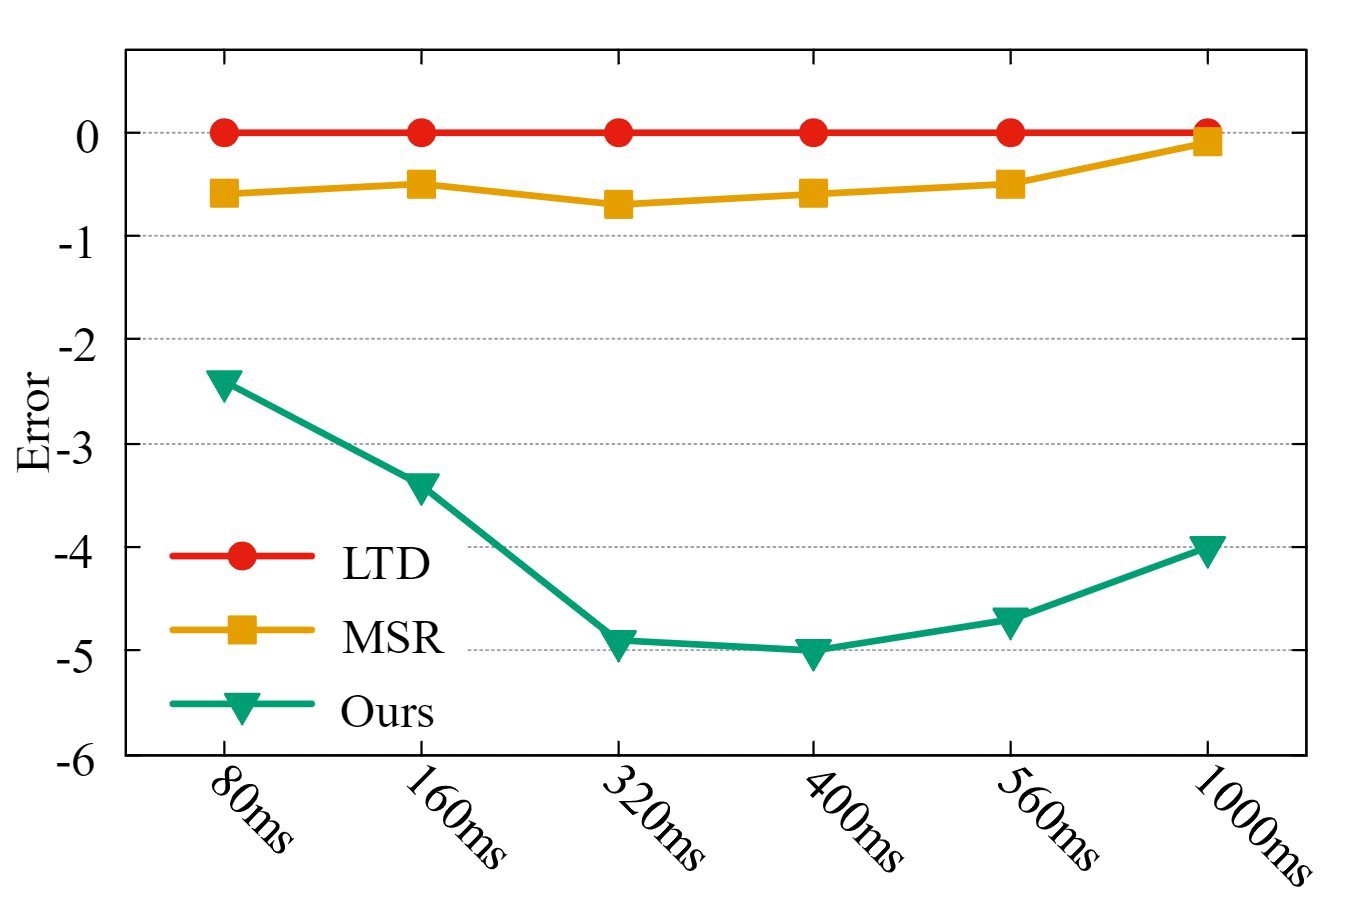
\includegraphics[width=0.60\textwidth]{FigMa/per_time.png}\\
    \vspace{-0.3cm}
    \caption{Human3.6M逐时刻相对误差对比}
    \label{fig:per_time_error}
\end{figure}

如图\ref{fig:per_time_error}所示,本文筛选了LTD,MSR这两个性能较好的算法作为对比对象,以LTD为基准,对比本方法与它们在80ms,160,320ms,400ms,560ms,1000ms 六个时刻的预测误差。注意图中所表现的误差以相对误差的形式展示,例如,MSR所在的黄色折线和本方法所在的绿色折线都是通过计算与LTD之间的相对误差得到的,由于MSR和本方法预测误差均小于LTD,所以相对误差均为负数。某个时刻,图上所在的位置越靠下(相对误差负地更多)则说明预测精度越高。由图上可以看出,MSR虽然整体上预测误差略小于LTD,但领先幅度不大,二者误差折线较为靠近,且在1000ms时刻二者预测误差几乎持平,这反映了MSR在长时预测能力方面的不足。而本方法在预测精确性方面大幅领先上述两个方法,
\begin{figure}[h]
    \centering
    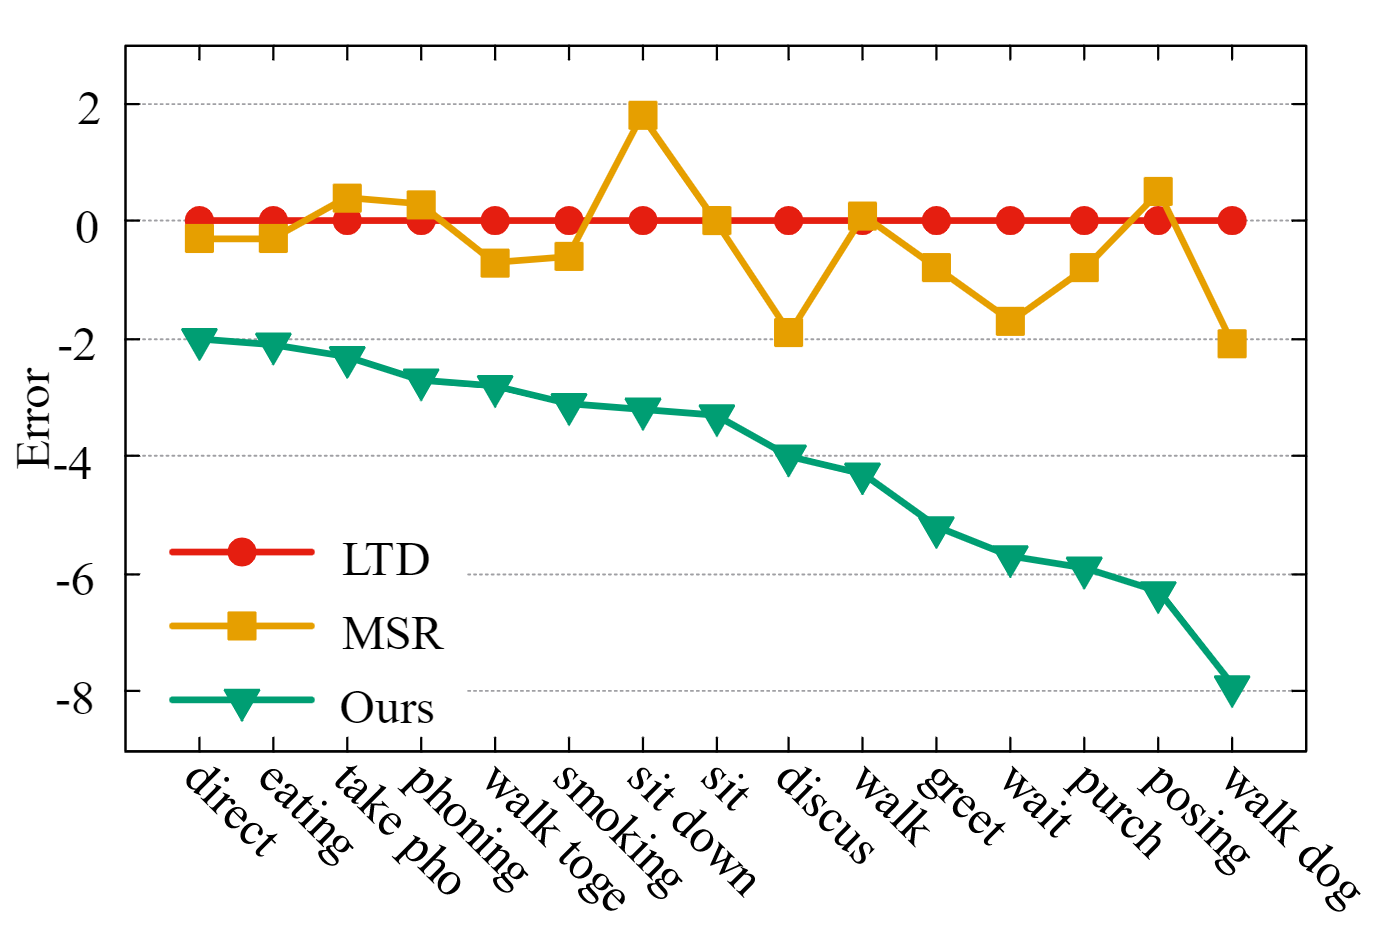
\includegraphics[width=0.60\textwidth]{FigMa/per_action.png}\\
    \vspace{-0.3cm}
    \caption{Human3.6M逐动作相对误差对比}
    \label{fig:per_action_error}
\end{figure}
平均领先约4个点。且在长时预测部分(560ms,1000ms)依然保持大幅领先,体现了本方法在长时依赖捕捉能力上的优势。


除了对逐时刻误差进行分析,本文还希望各个方法在不同的动作类别上的表现。类似的,在Human3.6M数据集上本文计算了不同动作类别上,各个方法间的相对误差。如图\ref{fig:per_action_error}所示,本文将动作类别按预测相对误差从小到大进行排序,从图中可以看到,MSR并没有体现对LTD的明显优势,甚至在部分动作(sitting down,taking photo)上还显著落后于LTD。而本文的方法在所有动作上都大幅领先MSR和LTD。在处理复杂动作,例如purchases,posing,walking dog上本文的领先幅度更加明显,这体现了本方法在处理复杂图结构关系上的优秀性能。

\begin{figure}[ht]
    \centering
    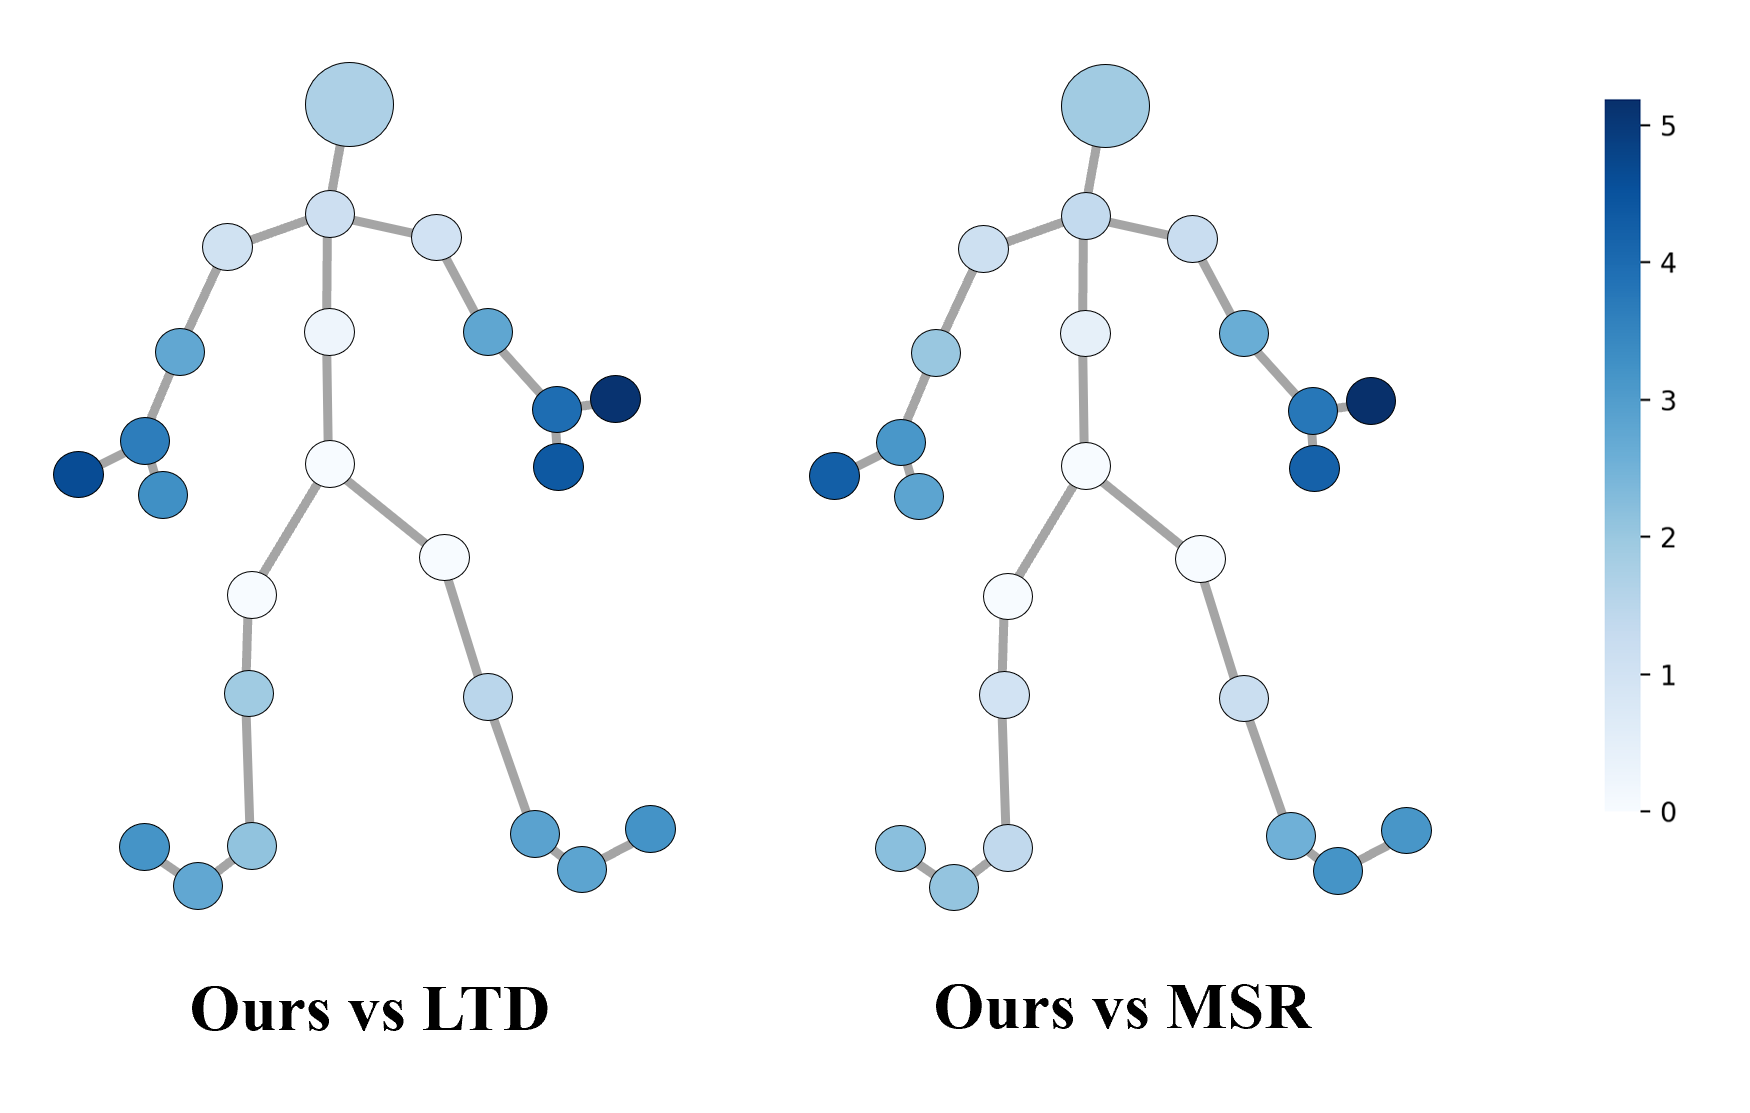
\includegraphics[width=0.60\textwidth]{FigMa/per_joint.png}\\
    \vspace{-0.3cm}
    \caption{Human3.6M逐关节点相对误差对比}
    \label{fig:per_joint_error}
\end{figure}

由于人体姿态中各个关节点的运动模式并不统一,模型对各个关节点的预测存在差异。因此,本文分析了各个关节点的预测误差。如图\ref{fig:per_joint_error}所示,本文对比了本方法与LTD(左)和MSR(右)在各个关节点上的相对预测误差。本文用各个关节点颜色的深浅程度代表相对误差的大小,颜色越深则说明在该关节点上本方法的预测误差越低。如图所示,由于MSR与LTD的性能相对接近,因此本方法与它们的相对误差结果也类似,表现在图中即,颜色分布情况基本相同。从两个人体姿态中可以看到,在运动模式较为稳定、简单的躯干部分,本方法领先程度较低,具体表现为关节点颜色较浅。而在运动模式较为复杂的躯体末端,如手臂,小腿等部分,本方法则提供了更加精确的预测结果。


\subsection{CMU-Mocap}


\begin{table*}[ht]
    \caption{CMU-Mocap上短时预测误差对比}
    \huge
    \renewcommand\arraystretch{1}
    \resizebox{\textwidth}{!}{
    \begin{tabular}{c|cccc|cccc|cccc|cccc}\hline
    scenarios    & \multicolumn{4}{c|}{basketball}                                & \multicolumn{4}{c|}{basketball signal}                       & \multicolumn{4}{c|}{directing traffic}                      & \multicolumn{4}{c}{jumping}                                   \\ \hline
    millisecond  & 80ms          & 160ms         & 320ms         & 400ms         & 80ms         & 160ms         & 320ms         & 400ms         & 80ms         & 160ms        & 320ms         & 400ms         & 80ms          & 160ms         & 320ms         & 400ms         \\ \hline
    Res. Sup. & 15.5          & 26.9          & 43.5          & 49.2          & 20.2         & 33.0          & 42.8          & 44.7          & 20.5         & 40.6         & 75.4          & 90.4          & 26.9          & 48.1          & 93.5          & 108.9         \\
    DMGNN        & 15.6          & 28.7          & 59.0          & 73.1          & 5.0          & 9.3           & 20.2          & 26.2          & 10.2         & 20.9         & 41.6          & 52.3          & 32.0          & 54.3          & 96.7          & 119.9         \\
    
    LTD          & 11.7          & 21.3          & 41.0          & 50.8          & 3.3          & 6.3           & 13.6          & 18.0          & 6.9          & 13.7         & 30.3          & 40.0          & 17.2          & 32.4          & 60.1          & 72.6          \\
    STSGCN      &28.4        &31.9         &48.2            & 64.6          &15.3      &15.4    &21.6      &35.5        &20.9         &22.6           &36.0            &58.3                &32.2           &41.4          &68.0      &86.1 \\ 
    MSR          & \underline{10.3}          & \underline{18.9}          & \underline{37.7}          & \underline{47.0}          & \underline{3.0}          & \underline{5.7}           & \underline{12.4}          & \underline{16.3}          & \underline{5.9}          & \underline{12.1}         & \underline{28.4}          & \underline{38.0}          & \underline{15.0}          & \underline{28.7}          & \underline{55.9}          & \underline{69.1}          \\
    Ours          & \textbf{9.5}  & \textbf{17.5} & \textbf{35.3} & \textbf{44.2} & \textbf{2.7} & \textbf{4.9}  & \textbf{10.8} & \textbf{14.6} & \textbf{4.8} & \textbf{9.8} & \textbf{23.6} & \textbf{32.3} & \textbf{13.9} & \textbf{27.8} & \textbf{55.8} & \textbf{69.0} \\ \hline
    scenarios    & \multicolumn{4}{c|}{soccer}                                    & \multicolumn{4}{c|}{walking}                                  & \multicolumn{4}{c|}{wash window}                              & \multicolumn{4}{c}{average}                                   \\ \hline
    millisecond  & 80ms          & 160ms         & 320ms         & 400ms         & 80ms         & 160ms         & 320ms         & 400ms         & 80ms         & 160ms        & 320ms         & 400ms         & 80ms          & 160ms         & 320ms         & 400ms         \\ \hline
    Res. Sup. & 17.8          & 31.3          & 52.6          & 61.4          & 44.4         & 76.7          & 126.8         & 151.4         & 22.8         & 44.7         & 86.8          & 104.7         & 24.0          & 43.0          & 74.5          & 87.2          \\
    DMGNN        & 14.9          & 25.3          & 52.2          & 65.4          & 9.6          & 15.5          & 26.0          & 30.4          & 7.9          & 14.7         & 33.3          & 44.2          & 13.6          & 24.1          & 47.0          & 58.8          \\
    
    LTD          & 13.3          & 24.0          & 43.8          & 53.2          & 6.6          & 10.7          & \underline{17.4}          & \underline{20.4}          & 6.0          & 11.6         & \underline{24.8}          & \underline{31.6}          & 9.3           & 17.1          & 33.0          & 40.9          \\
    
    STSGCN      &31.2      &34.8            &53.1           &73.2           &21.9                     &21.4         &25.9           &38.9               &17.6      &19.2                    &30.9      &53.5      &25.3         &27.9           &41.8      &59.2 \\
    MSR          & \textbf{10.9} & \textbf{19.5} & \textbf{37.1} & \textbf{46.4} & \underline{6.3}          & \underline{10.3}          & 17.6          & 21.1          & \underline{5.5}          & \underline{11.1}         & 25.1          & 32.5          & \underline{8.1}           & \underline{15.2}          & \underline{30.6}          & \underline{38.6}          \\
    Ours          & \underline{11.1}          & \underline{20.6}          & \underline{39.5}          & \underline{48.7}          & \textbf{6.2} & \textbf{10.3} & \textbf{16.8} & \textbf{19.8} & \textbf{4.6} & \textbf{9.2} & \textbf{20.9} & \textbf{27.3} & \textbf{7.6}  & \textbf{14.3}  & \textbf{29.0} & \textbf{36.6} \\ \hline
    \end{tabular} 
    }
    \label{table:CMU_short_term}
    \end{table*}
    
    \begin{table}[ht]
    \caption{CMU-Mocap上的长时预测误差对比}
    \huge
    \renewcommand\arraystretch{1.0}
    \resizebox{1.0\columnwidth}{!}{
    \begin{tabular}{c|cc|cc|cc|cc|cc|cc|cc|cc} \hline
    scenarios    & \multicolumn{2}{c|}{basketball} & \multicolumn{2}{c|}{basketball signal} & \multicolumn{2}{c|}{directing traffic} & \multicolumn{2}{c|}{jumping}    & \multicolumn{2}{c|}{soccer}      & \multicolumn{2}{c|}{walking}   & \multicolumn{2}{c|}{wash window} & \multicolumn{2}{c}{average}   \\ \hline
    millisecond  & 560ms          & 1000ms        & 560ms             & 1000ms            & 560ms             & 1000ms            & 560ms         & 1000ms         & 560ms          & 1000ms         & 560ms         & 1000ms        & 560ms          & 1000ms         & 560ms         & 1000ms        \\ \hline
    Res. Sup. & \textbf{54.3}  & \textbf{72.8} & 51.4              & 60.6              & 112.9             & 153.1             & 128.8         & 162.8          & 72.33          & 107.37         & 182.4         & 194.3         & 136.3          & 202.7          & 105.5         & 136.3         \\
    DMGNN        & 96.1           & 138.6         & 36.6              & 52.0              & 72.3              & 111.2             & 160.6         & 224.6          & 82.22          & 111.90         & 37.8          & 67.0          & 56.5           & 82.8           & 77.4          & 112.6         \\
    LDT          & 68.1           & 98.0          & 27.7              & 54.0              & 60.9              & 114.2             & 93.8          & 127.4          & 70.85          & 108.26         & \underline{25.2}    & \underline{34.4}    & \underline{43.9}     & \underline{67.0}     & 55.8          & 86.2          \\
    STS-GCN              & 75.3                 & 109.2                & 38.7                 & 63.5                 & 66.7                 & 113.4                & 102.6                & 135.1                & 84.9                 & 116.6                & 39.0                 & 46.1                 & 51.6                 & 79.2                 & 65.5                 & 94.7 \\
    MSR          & 62.8           & 87.0          & \underline{24.6}        & \textbf{47.9}     & \underline{58.9}        & \underline{111.0}       & \underline{92.1}    & \textbf{124.8} & \textbf{64.41} & \textbf{99.32} & 27.2          & 39.7          & 45.9           & 71.3           & \underline{53.7}    & \underline{83.0}    \\
    Our          & \underline{59.4}     & \underline{84.1}    & \textbf{23.7}     & \underline{50.2}        & \textbf{51.6}     & \textbf{102.3}    & \textbf{91.7} & \underline{125.6}    & \underline{65.4}     & \underline{99.0}     & \textbf{25.1} & \textbf{33.9} & \textbf{39.7}  & \textbf{65.7}  & \textbf{50.9} & \textbf{80.1} \\ \hline
    \end{tabular}
    }
    \label{table:CMU_long_term}
    \end{table}

对于CMU-Mocap数据集,与Human3.6M类似,本文分别在短时预测(输入10帧预测10帧)和长时预测(输入10帧预测25帧)两种情况下与现有方法进行对比。表\ref{table:CMU_short_term}展示了短时预测结果,本文同样选取80ms,160ms,320ms,400ms四个时刻进行对比,从表中可以看出,本方法依然延续了在预测精度方面的优势,在加粗的最优结果和下划线的次优结果数量上远远超过现有方法。表\ref{table:CMU_long_term}展示了长时预测结果,本文依旧拥有最多的最优和次优结果,在预测平均指标(50.9,80.1)上也明显领先现有次优方法(53.7,83.0)。以上内容说明在CMU-Mocap数据集中,本方法在预测精确性上相较现有方法依然保持了明显的领先。

\begin{table}[ht]
    \caption{3DPW上的长短时预测误差对比}
    \huge
    \centering
    \renewcommand\arraystretch{0.7}
    \resizebox{0.5\columnwidth}{!}{
    \begin{tabular}{c|ccccc} \hline
    millisecond      & 200ms         & 400ms         & 600ms         & 800ms         & 1000ms         \\ \hline
    Res. Sup.    & 113.9         & 173.1         & 191.9         & 201.1         & 210.7          \\
    DMGNN  &37.3  &67.8  &94.5  &109.7  &123.6 \\
    LTD       & {35.6}          & {67.8}          & {90.6}          & {106.9}         & {117.8}          \\
    STS-GCN  &\underline{35.1}  &\underline{66.2}  &\underline{87.0}  &\underline{101.4}  &\underline{112.2} \\
    MSR        & {37.8}          & {71.3}          & {93.9}          & {110.8}          & {121.5}          \\
    Ours        & \textbf{29.3}& \textbf{58.3} & \textbf{79.8} & \textbf{94.4}  & \textbf{104.1} \\ \hline
    \end{tabular}
    }
    \label{table:3DPW_shortlong}
    \end{table}

\subsection{3DPW}
在3DPW数据集上进行的对比与上述两个数据集有所不同。为了统一对比条件,本文参考了\parencite{mao2019learning}中的实验设置,在输入10帧预测30帧的模型上统计长时和短时预测误差,取200ms,400ms,600ms,800ms,1000ms五个时刻计算预测误差。此外,由于3DPW不区分动作类别,本文只统计了整个数据集上的预测误差。最终,在3DPW数据集上,本文在所有时刻的预测误差对比中都提供了最精确的结果,且远远超过次优的结果。


\section{预测结果定性对比}
在第\ref{section:prediction_error}节中,本文在三个公开数据集上将本方法与现有方法的模型精确性进行了对比,结果显示本方法在三个数据集的预测误差均远小于现有方法。同时,本文还考察了时序、动作类别和关节点类别对预测结果的影响,结果显示本方法具有较强的时序信息处理能力,在长时预测、复杂动作和高频率运动关节点预测方面有较大优势。然而数值上的差异很难带来直观上的感受。因此,本文在图\ref{fig:prediction_result}中展示定性的对比结果。

\begin{figure}[ht]
    \centering
    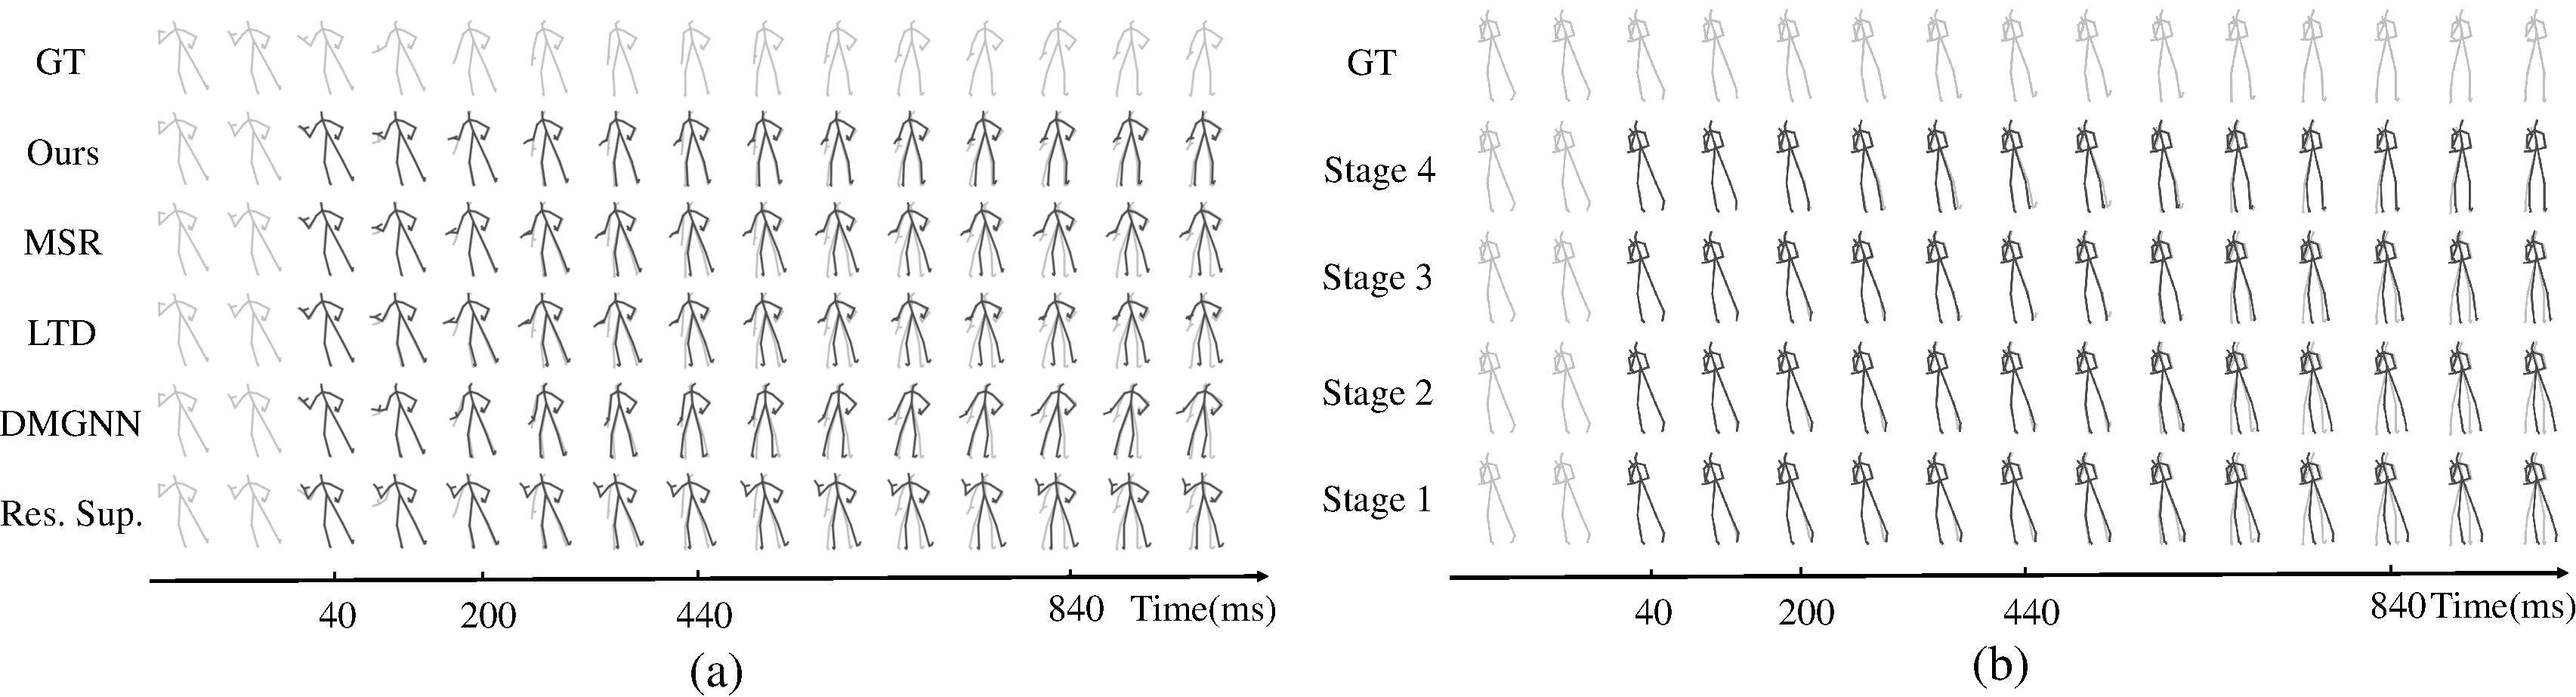
\includegraphics[width=1\textwidth]{FigMa/prediction_result.pdf}\\
    \vspace{-0.3cm}
    \caption{人体运动姿态预测对比}
    \label{fig:prediction_result}
\end{figure}

在图\ref{fig:prediction_result}(a)中,本文选取了Res. Sup.,DMGNN,LTD和MSR作为对比对象。图中第一行为真值,以浅灰色表示。第二行为本方法的预测结果,前两个灰色人体姿态为网络已知的输入,随后的黑色人体姿态为1000ms内的待预测的未来人体运动姿态,本文用黑色表示预测结果,浅灰色为真值,二者的重合程度越高则说明预测误差越小。其他方法也使用了类似的展示方法。从图\ref{fig:prediction_result}(a)中可以看到本文的方法是五个方法中预测结果与真值重合度最高的,其他方法从上往下预测误差逐渐增加,且随着时间前进误差越来越大。\ref{fig:prediction_result}(b)中则展示了网络不同阶段的预测结果。可以看到,第一阶段的结果较为粗糙只预测了运动的大致趋势,而随着网络逐渐深入,预测结果也逐渐向真值靠近。图\ref{fig:more_result}提供了不同动作的对比结果,图\ref{fig:SMPL}则展示了部分由SMPL\parencite{loper2015smpl}渲染的结果。


\begin{figure*}[ht]
    \centering
    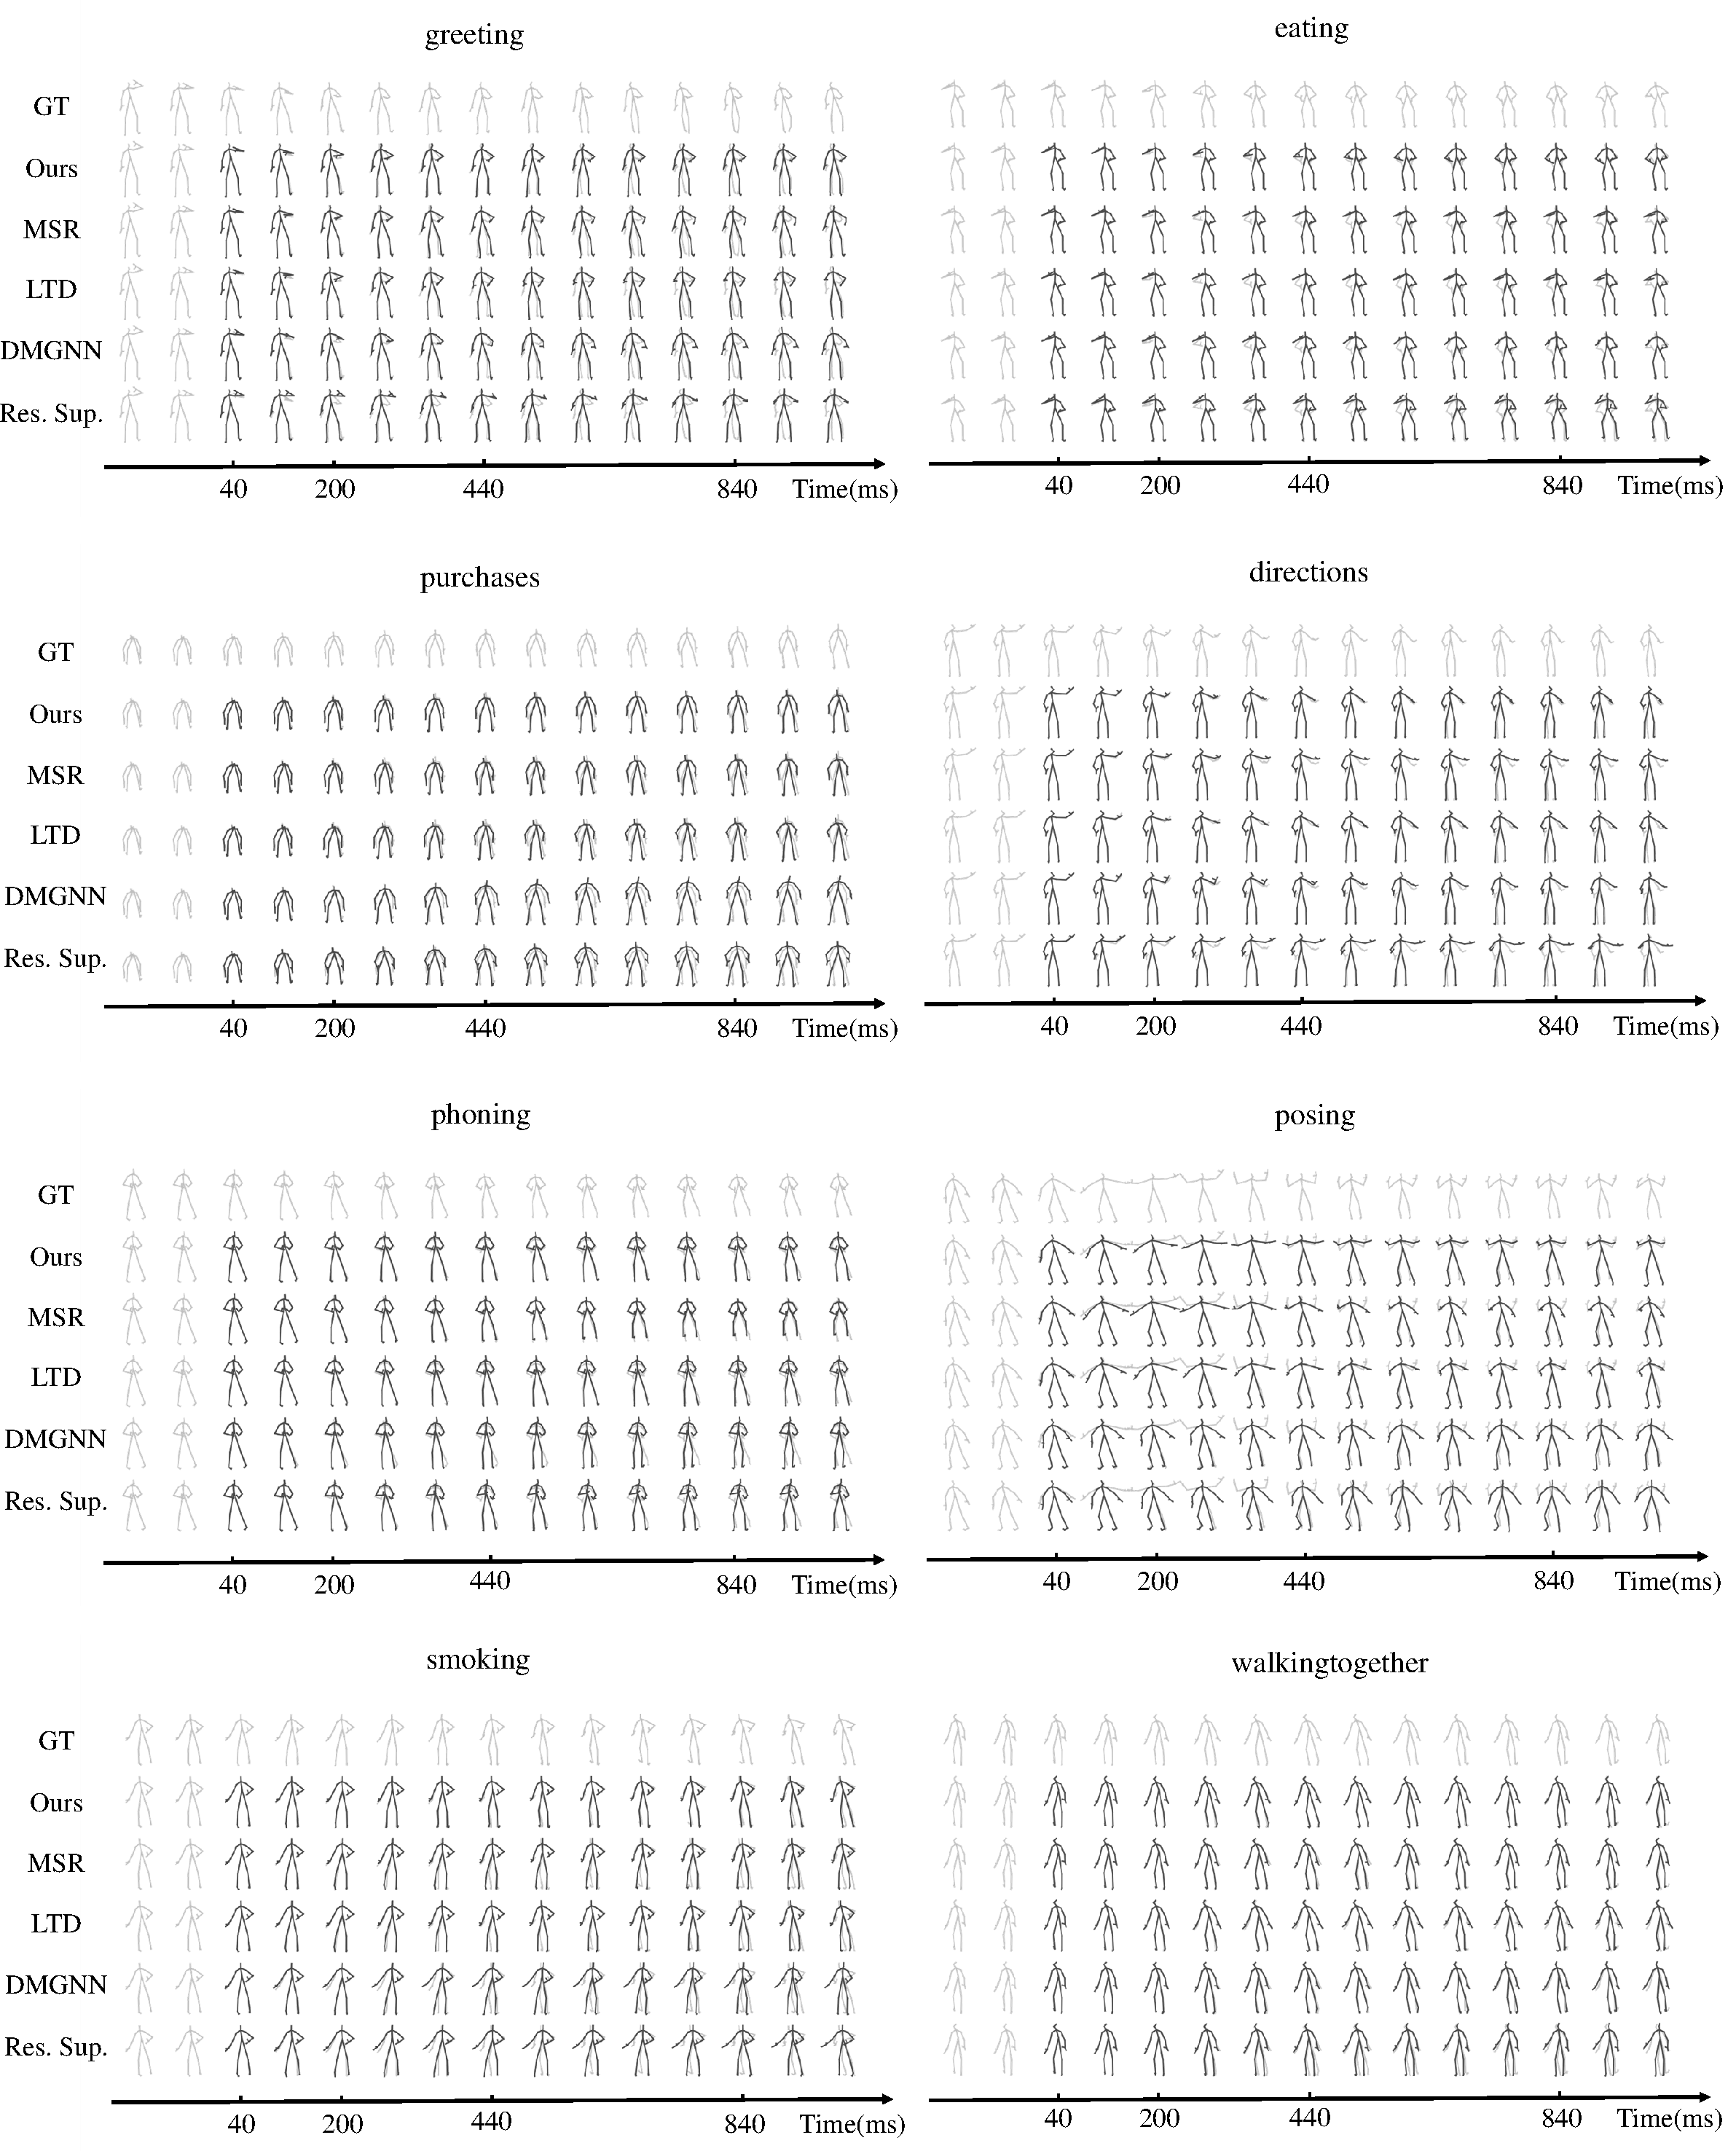
\includegraphics[width=1\textwidth]{FigMa/more_result.pdf}
    \caption{Human3.6M中各动作的可视化预测结果}
    \label{fig:more_result}
\end{figure*}

\begin{figure*}[ht]
    \centering
    \includegraphics[width=1\textwidth]{FigMa/SMPL.pdf}
    \caption{Human3.6M中各动作的SMPL格式可视化预测结果}
    \label{fig:SMPL}
\end{figure*}

\clearpage

\section{消融实验}
在上述两个章节中本文从定性和定量两个角度对本方法的预测精确性进行了分析。在本章节中,本文将通过控制变量法,对网络中各个模块进行有效性分析。具体的,本文将从三个方面进行实验。第一是对多阶段网络结构进行分析,探索其相对现有单阶段网络的优势,以及网络超参数设置的逻辑。第二是对中级监督目标进行分析,本文将首先尝试验证中级监督目标在训练过程中发挥的积极作用,随后通过对比实验,验证本方法提出的累积均值平滑策略相对现有平滑方法的优势。第三则是对ST-DGCN图卷积模块的分析,本文将在保持网络原有结构不变的前提下,将ST-DGCN模块替换为其他方法中的图卷积。并评估它们对预测精度的影响。需要注意的是,本章所有实验均在Human3.6M数据集上进行。
\subsection{对多阶段网络结构的分析}
本文首先进行对多阶段网络结构的分析,本文考虑在保持网络其他部分不变的前提下,将多阶段网络修改为单阶段网络是否会造成不良影响。具体的,本文选择提取出多阶段模型中的一个阶段将其中的GCB数量从3增加到12,同时去掉网络中的中级监督,以此在保证网络中特征提取模块GCB数量一致的情况下,将多阶段网络修改为单阶段网络。实验结果如下所示:

\begin{table*}[h]
    \begin{center}
    \resizebox{1\textwidth}{!}{
    \begin{tabular}{c|c|cccccccc|c} \hline
                              \multicolumn{2}{c|}{对比方法}      & 80ms           & 160ms                           & 320ms                           & 400ms                           & 560ms                           & 720ms                           & 880ms                            & 1000ms                           & 平均误差                         \\ \hline
                              \multicolumn{2}{c|}{单阶段网络  }           & 11.95          & 24.47                           & 49.69                           & 60.94                           & 79.56                           & 93.93                           & 105.86                           & 113.41                           & 67.48                           \\ \hline
                              \multicolumn{2}{c|}{本方法}                          & \textbf{10.33} & \textbf{22.74} & \textbf{47.45} & \textbf{58.46} & \textbf{76.91} & \textbf{91.20} & \textbf{102.77} & \textbf{110.31} & \textbf{65.02} \\ \hline
    \end{tabular}
    }
    \end{center}
    \caption{单阶段网络与多阶段网络对比}
    \label{table:ablation_1}
    \end{table*}

表\ref{table:ablation_1}展示了单阶段网络和多阶段网络在8个时刻的预测误差对比。可以看出本方法中的多阶段网络在各个时刻的预测误差都显著低于单阶段版本。这体现了通过拆分预测目标所带来的预测不确定性降低的优点。

另外,在多阶段网络结构中,阶段数量这一超参数的设置也需要通过实验验证来确定。具体的,本文设置了如下实验来搜索最优的网络阶段数:在保持网络始终拥有12个GCB的前提下,本文通过调整每个阶段包含的GCB数量来调整阶段数量。例如,如果将每个阶段包含的GCB数量从3个增加到4个,则网络中包含的阶段数量也从4个下降到3个。值得注意的是,中级监督目标的数量与网络阶段数一致,网络阶段数的变化也会导致中级监督目标数量的改变。
\begin{figure}[ht]
    \centering
    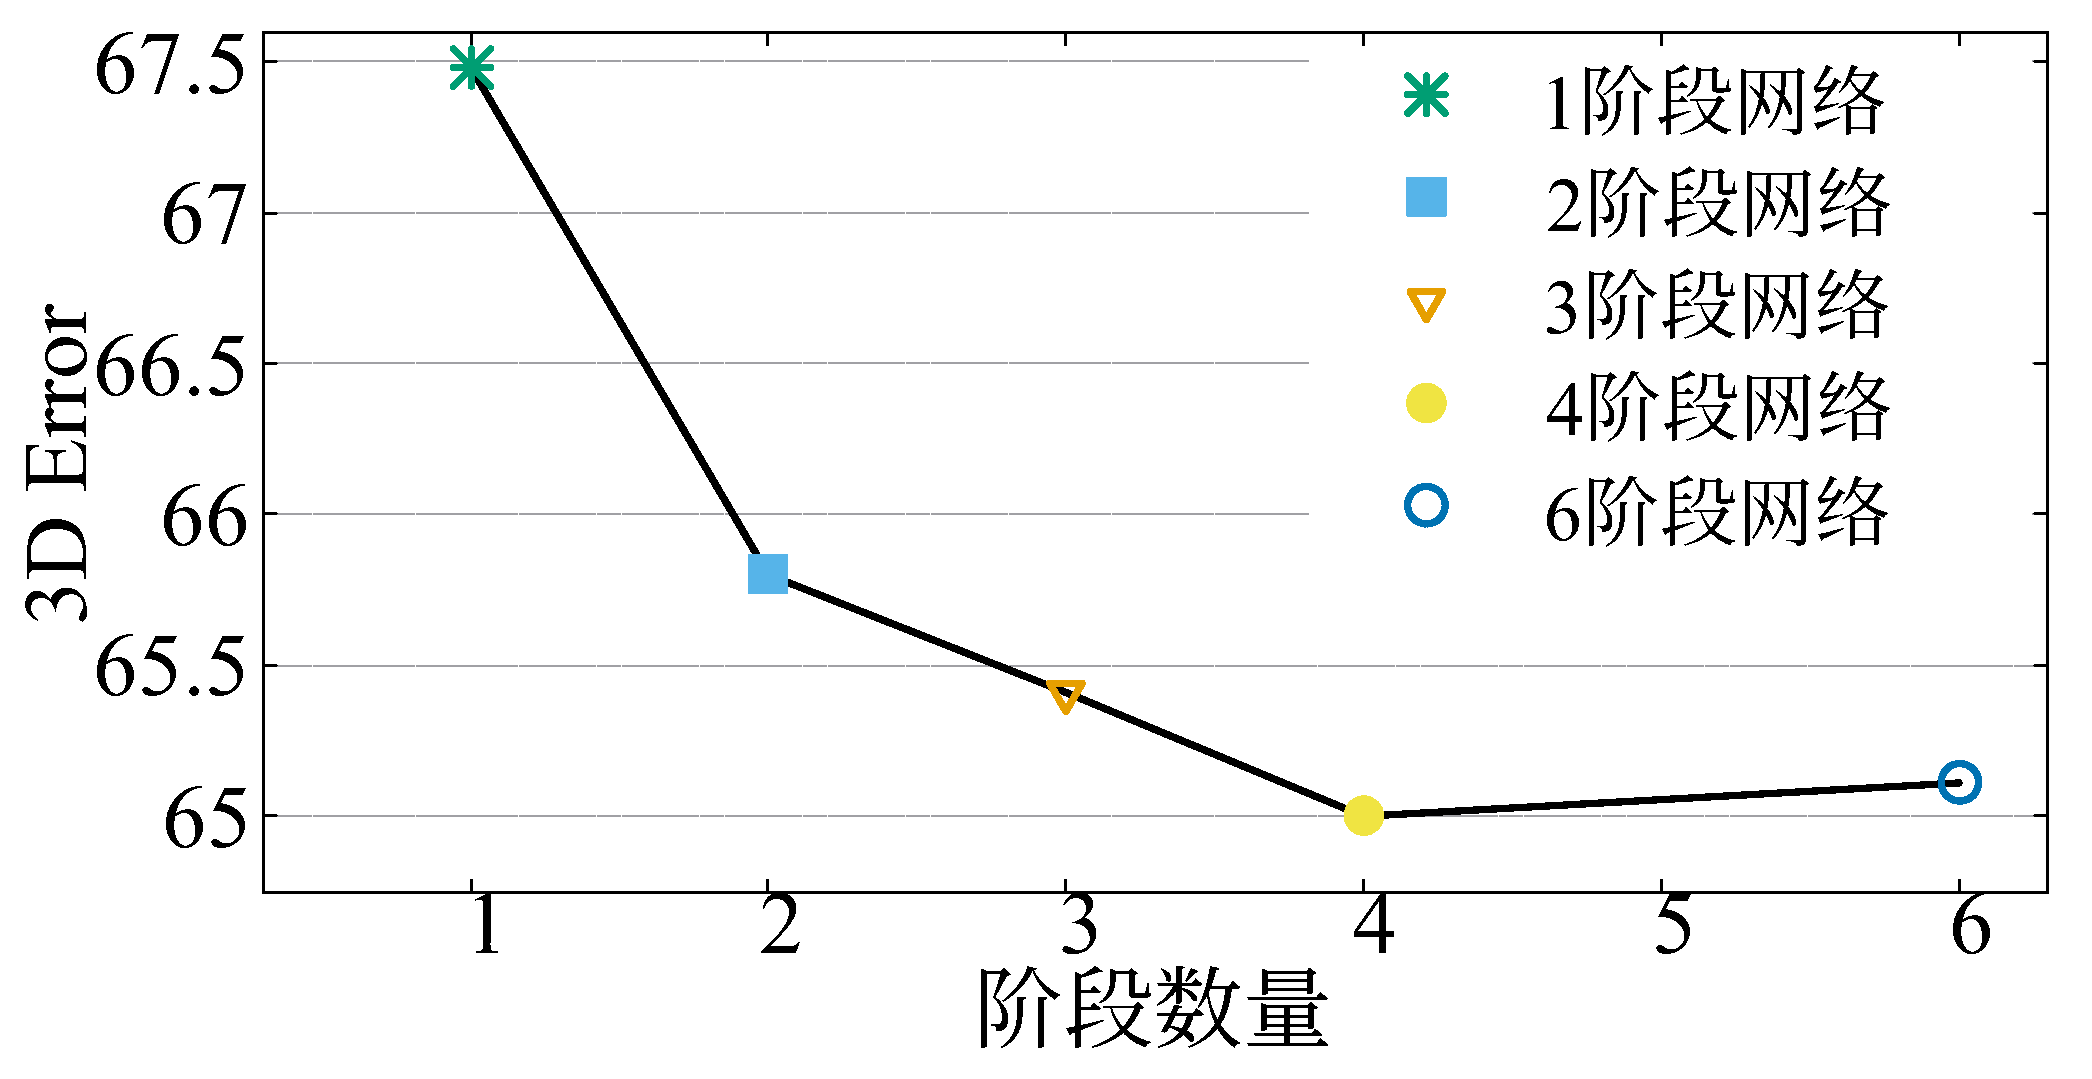
\includegraphics[width=0.6\columnwidth]{FigMa/smooth_stage_chinese.pdf} \\
    \caption{阶段数量对预测结果的影响}
    \label{fig:ablation-stage-number}
\end{figure}

图\ref{fig:ablation-stage-number}展示了不同的阶段数量对网络预测平均误差的影响。由于网络中的GCB总数被确定为12个(参考LTD的设置),且每个阶段的GCB数量必须保持一致。所以本文测试了阶段数量分别为1,2,3,4,6 时的情况。从图中可以看出,当阶段数量从1增加到4时,网络的预测误差逐步下降,这是由于多阶段的预测降低了预测不确定性,且预测目标被分的越细,每个阶段的预测难度也越低。但当阶段数量从1增加到4时,预测误差非但不下降,反而还有所上升,这是由于多阶段网络复杂度的提升抵消了这部分增益。因此,在本文的网络中,阶段数量被设置为4。

\subsection{对中级监督目标的分析}
本文中提到的中级监督目标构造方法(累积均值平滑)是本文的一个重要创新。在多阶段网络中,好的中级监督目标可以帮助网络建立层次化的预测过程,降低预测中的歧义和不确定性。而差的中级监督目标会导致不同阶段预测目标过渡不平滑,对预测产生负面影响。因此有必要分析各种中级监督目标对预测精确度的影响。

\begin{table*}[ht]
    \begin{center}
    \resizebox{1\textwidth}{!}{
        \begin{tabular}{c|c|cccccccc|c} \hline
            \multicolumn{2}{c|}{对比方法}      & 80ms           & 160ms                           & 320ms                           & 400ms                           & 560ms                           & 720ms                           & 880ms                            & 1000ms                           & 平均误差                         \\ \hline
            \multicolumn{2}{c|}{去除中级监督}            & 11.42          & 24.02                           & 49.73                           & 60.94                           & 79.49                           & 93.45                           & 105.12                           & 112.42                           & 67.07                           \\ 
            \multicolumn{2}{c|}{将真值作为中级监督}    & 11.04          & 23.49                           & 48.83                           & 59.89                           & 78.13                           & 92.2                & 103.87                           & 111.46                           & 66.11                           \\ 
            \multicolumn{2}{c|}{将高斯平滑作为中级监督} &12.04	&24.36	&49.80	&60.90	&78.67	&92.19	&103.51	&110.98 &66.55
\\ \hline
\multicolumn{2}{c|}{本方法}                         & \textbf{10.33} & \textbf{22.74} & \textbf{47.45} & \textbf{58.46} & \textbf{76.91} & \textbf{91.20} & \textbf{102.77} & \textbf{110.31} & \textbf{65.02} \\ \hline
\end{tabular}
    }
    \end{center}
    \caption{不同中级监督目标对预测误差的影响}
    \label{table:ablation_2}
    \end{table*}

表\ref{table:ablation_2}展示了不同中级监督目标对预测误差的影响,第一行为去掉所有的中级监督目标只保留真值对网络最终输出的监督。它将作为基准网络来体现各种中级监督目标对网络的影响。第二行为使用真值作为所有阶段的中级监督目标,第三行为用高斯平滑构建中级监督目标。从表中可以看到,使用累积均值平滑(AAS)的本方法相比较上述的三种方案有明显优势。其中第一行为不使用中级监督目标,预测精度最差,与现有的单阶段网络无异。第二行使用真值作为所有阶段的中级监督目标,相较于不使用中级监督,精度有一定提升。第三行使用通过高斯平滑的中级监督目标,效果介于上述二者之间,这是由于使用该方法处理的关节点轨迹中存在过渡部分不连续的情况,影响了网络的最终预测精确性。而本文提出的累积均值平滑在预测精度上明显超过了上述三个样本,证明了AAS可以在多阶段网络中建立层次化的预测过程,有效降低了预测不确定性。

\subsection{对ST-DGCN图卷积模块的分析}\label{section:gcn_block}
除了对多阶段网络结构展开分析,本文还希望替换网络中的图卷积模块来证明本方法中提出的ST-DGCN的优势。具体的,在保持网络其他部分不变的前提下,本文使用\ref{section:ST-DGCN}章中,提到的Full \ spatiotemporal \ GCN、ST-GCN\parencite{yan2018spatial}、LTD\parencite{mao2019learning}和STS-GCN\parencite{sofianos2021space}中的GCN替换网络中的ST-DGCN。本文希望通过对比以上图卷积模块的预测精确性来证明ST-DGCN的出色性能。

\begin{table*}[ht]
    \begin{center}
    \resizebox{1\textwidth}{!}{
    \begin{tabular}{c|c|cccccccc|c} \hline
                              \multicolumn{2}{c|}{对比方法}      & 80ms           & 160ms                           & 320ms                           & 400ms                           & 560ms                           & 720ms                           & 880ms                            & 1000ms                           & 平均误差                         \\ \hline
                              \multicolumn{2}{c|}{在我们的模型中使用full spatiotemporal GCN}  &12.92	&26.51	&52.85	&64.06	&82.01	&95.64	&106.92	&114.25 &69.40\\
                              \multicolumn{2}{c|}{在我们的模型中使用 ST-GCN\parencite{yan2018mt}}& 11.84          & 25.78                           & 51.87                           & 62.73                           & 80.23                           & 93.61                           & 105.00                              & 112.72                           & 67.97                           \\ 
                              \multicolumn{2}{c|}{在我们的模型中使用LTD \parencite{mao2019learning}的DCT-GCN}  & 11.11          & 24.01                           & 49.48                           & 60.67                           & 79.34                           & 93.91                           & 105.55                           & 113.1                            & 67.15                           \\ 
                              \multicolumn{2}{c|}{在我们的模型中使用STS-GCN \parencite{sofianos2021space}} &10.78	&23.48	&49.38	&60.88	&80.08	&95.14	&107.19	&114.52 &67.68\\ \hline
    
     
                              \multicolumn{2}{c|}{本方法}                         & \textbf{10.33} & \textbf{22.74} & \textbf{47.45} & \textbf{58.46} & \textbf{76.91} & \textbf{91.20} & \textbf{102.77} & \textbf{110.31} & \textbf{65.02} \\ \hline
    \end{tabular}
    }
    \end{center}
    \caption{不同图卷积模块对预测误差的影响}
    \label{table:ablation_3}
    \end{table*}
    
表\ref{table:ablation_3}展示了本文的ST-DGCN和其他四种图卷积模块的预测误差对比结果。从图中可以看到ST-DGCN的预测精度遥遥领先其余四个方法。最差的结果是Full \ spatiotemporal \ GCN,这和本文的分析一致,虽然它通过同时对数据的时间和空间维度进行建模,使得模型拥有了直接的时空信息感知能力,但过度膨胀的邻接矩阵给训练和推理过程带来了负面影响。其次是ST-GCN和STS-GCN,他们都采用了时空分离的策略来降低邻接关系复杂度,但前者受限于时间上的局部感受野,后者受限于冗余的网络结构,只达到了有限的提升。LTD则使用GCN对空间维度进行建模,通过DCT将时序数据变换到频率域在进行处理,拥有了第二低的预测误差。而本文的ST-DGCN综合了以上方法的优点,在提高网络时序依赖捕捉能力的同时,使用时空分离策略提高了效率,达到了最低的预测误差。

\section{时间效率分析}
在上述实验中,本文着重分析了模型中不同模块对于预测精度的影响,以验证本方法中各模块在设计上的可行性。在衡量模型综合性能的过程中,除了分析预测精确度,模型执行效率和空间占用也是一个极为重要的指标。因此在本节,本文将对本方法的时间和空间效率进行对比分析。

\begin{table}[ht]
    \centering
    \resizebox{0.7\textwidth}{!}{
    \begin{tabular}{c|c|c|c} \hline
    对比方法      & 训练阶段 (每个batch) & 推理阶段 (每个batch) & 模型尺寸 \\ \hline
    DMGNN       & 473ms            & 85ms            & 46.90M         \\ 
    LTD         & 114ms            & 30ms            & 2.55M          \\  
    STS-GCN      & 12.2ms             & 2.8ms           & 0.058M         \\ 
    MSR         & 191ms            & 57ms            & 6.30M          \\ \hline
    本方法的多阶段模型 (使用full spatiotemporal GCN) &221ms &54ms &67.99M \\
    本方法的多阶段模型 (使用ST-GCN\parencite{yan2018spatial}) &132ms &38ms &1.54M \\ 
    本方法的多阶段模型 (使用STS-GCN\parencite{sofianos2021space}) &182ms &49ms &5.69M \\ \hline
    本方法         & 145ms            & 43ms            & 1.74M          \\ \hline
    \end{tabular}
    }
    \caption{时间效率和模型空间占用对比}\label{table:ablation-efficiency}
    \end{table}
由于不同数据集中人体运动姿态序列的空间结构和预测时序长度都对网络运行时间和模型空间占用有所影响。本文统一在Human3.6M长时预测实验环境下,统计每种方法执行一个Batch所使用的时间(BatchSize 16)以及模型参数量。统计结果如表\ref{table:ablation-efficiency}中所示。表格被纵向分割为三个区域,本文的模型位于最下面的区域。自上而下第一个部分是现有方法训练推理时间和模型空间占用(单位为M)。可以看到本方法的时间效率和空间效率都属于靠前的位置。由于部分图卷积模块并没被直接应用于人体运动姿态问题中。因此本文仿照第\ref{section:gcn_block}节,用上述图卷积网络替换本方法中的ST-DGCN后再进行统计,从第二个区域的结果中可以看到,与现有图卷积模块对比,本方法在时间和空间综合性能上任然不落下风。

通过上述实验证明,本方法在预测精度和时间、空间效率两个方面全面领先现有方法。

\section{总结}
在本章节中,本文通过实验证明了本方法在预测精度和执行效率这两个综合指标上全面领先现有方法,此外本文还通过消融实验详细分析了多阶段网络结构和ST-DGCN的设计有效性,验证了本方案的合理性。

具体的,本文首先介绍了本方法具体的实现细节,超参数设计以及运行环境等实验环境。随后本文介绍了实验中使用的三个公开数据集(Human3.6M,CMU-Mocap,3DPW)包括它们的制作者、记录方法、数据结构、数据格式等信息。此外,现有方法对不同数据集的特殊处理及统计方法也在文中有所提及。随后本文介绍了参与对比实验的各个现有方法,挑选不同种类,目前具有代表性5个性能达到SOTA的方法作为主要对比对象。在进行定量对比实验之前,介绍了在实验过程使用的预测精确度,测试指标—MPJPE(Mean Per-Joint Position Error),并给出了该指标的定义方式和实验中的测试方法。

在定量对比部分,本文在三个公开数据集上,使用通用的度量指标和公开代码或预训练模型,计算各个方法在不同的动作类型中逐时刻的3D预测误差。结果显示,本方法在三个数据集上全面领先现有的5个方法。除了数值上的定量对比,本文还进行了直观的定性对比,展示以人体骨架、SMPL模型为形式的人体运动姿态序列预测结果,从直观的结果上来,本方法的预测误差也显著低于现有方法。在证明本方法在预测精度上的优势后。本文还在随后的消融实验中对多阶段网络结构,累积均值平滑策略,ST-DGCN模块进行了对比分析,证明了以上设计的有效性和相对现有方法的优秀性能,最后本文还对本模型的时间、空间效率进行了对比,结果显示,在模型执行效率上,本方法仍然不落下风。

最后,根据实验结果,本文得出结论,本方法在预测精确度和运行效率方法均领先现有方法,且网络中各个模块的性能也达到了本文的设计期望,这使得本方法成为人体运动姿态预测领域新的SOTA算法。

